\documentclass[iop,apj,twocolappendix,numberedappendix]{emulateapj}
\usepackage{amsmath,amssymb,amstext}

\usepackage[breaklinks,colorlinks,citecolor=blue,linkcolor=magenta]{hyperref}
\usepackage[all]{hypcap} %Links go to figures; breaks on deluxetables (use \capstartfalse \capstarttrue to fix it)

\newlength{\colwidth}
\setlength{\colwidth}{\columnwidth}

\addtolength\voffset{0.8cm}

%% LLT: Adding these manually so that they're already defined
%% during the very first compile
%% Need each line for each table
\makeatletter
\def\deluxe@table@width@i{0pt}
\def\deluxe@table@width@ii{0pt}
\def\deluxe@table@width@iii{0pt}
\makeatother


\newcommand{\ds}{\displaystyle}
\newcommand{\be}{\begin{equation}}
\newcommand{\ee}{\end{equation}}
\newcommand{\bee}{\begin{eqnarray}}
\newcommand{\eee}{\end{eqnarray}}

\newcommand{\ov}{ \Omega_{\rm \Lambda} }
\newcommand{\om}{ \Omega_{\rm m} }
\newcommand{\mob}{ M_{\rm obj} }
\newcommand{\mstar}{ M_{*}(a) }
\newcommand{\msol}{\hbox{${\rm M}_\odot$}}

\newcommand{\rvir}{\hbox{$r_{\rm 200}$}}
\newcommand{\mvir}{\hbox{$M_{\rm vir}$}}
\newcommand{\Mvir}{\hbox{$M_{\rm vir}$}}
\newcommand{\vvir}{\hbox{$v_{\rm 200}$}}
\newcommand{\tvir}{T_{\rm vir}}
\newcommand{\mthresh}{M_{\rm t}}
\newcommand{\nsats}{n_{\rm sats}}
\newcommand{\vmax}{{\rm v}_{\rm max}}
\newcommand{\zreion}{z_{\rm reion}}
\newcommand{\LCDM}{$\Lambda$CDM }
\newcommand{\sigate}{ \sigma_{8}}
\newcommand{\actoy}{a_{c,{\rm toy}}}
\newcommand{\K}{{\rm K}}


\newcommand{\DME}{D_{\rm M31}}
\newcommand{\vMEI}{v_{\rm M31}}
\newcommand{\MMEI}{M_{\rm M31}}
\newcommand{\DMEE}{D_{\rm M33}}
\newcommand{\vMEE}{v_{\rm M33}}
\newcommand{\MMEE}{M_{\rm M33}}
\newcommand{\DLMC}{D_{\rm LMC}}
\newcommand{\vLMC}{v_{\rm LMC}}
\newcommand{\MLMC}{M_{\rm LMC}}
\newcommand{\MMW}{{\rm M}_{\rm MW}}
\newcommand{\Nsubs}{N_{\rm subs}}


\newcommand{\LikePR}{\textbf{Pr(d$\vert$x)}}

\def\rx{X}
\def\ry{Y}
\def\rz{Z}
\def\vx{v_X}
\def\vy{v_Y}
\def\vz{v_Z}
\def\distance{D}
\def\vrad{v_{\rm rad}}
\def\vtan{v_{\rm tan}}

\def\pr{{\rm Pr}}
\def\pars{\mathbf{x}}
\def\parsi{x_i}
\def\data{\mathbf{d}}
\def\datai{d_i}
\def\datap{\mathbf{d}^{\rm p}(\pars)}
\def\datapi{d^{\rm p}_{i}(\pars)}

\newcommand{\Msun}{{\rm M}_\odot}
\newcommand{\hinv}{h^{-1}}
\newcommand{\Mpc}{{\rm Mpc}}
\newcommand{\hmpc}{\hinv\Mpc}
\newcommand{\kpc}{{\rm kpc}}
\newcommand{\kms}{{\rm km s}^{-1}}

\newcommand{\rhobar}{\langle \rho \rangle}
\newcommand{\sig}{ \langle \sigma v \rangle }
\newcommand{\sigwig}{ {\widetilde \sigma} }
\newcommand{\rbh}{ r_{\rm bh} }
\newcommand{\rmax}{ r_{\rm max} }
\newcommand{\kmsmpc}{\, \rm{km}\,  \rm{s}^{-1}\, \rm{Mpc}^{-1}}
\newcommand{\lsim}{\lower.5ex\hbox{\ltsima}}
\newcommand{\gsim}{\lower.5ex\hbox{\gtsima}}
\newcommand{\ltsima}{$\; \buildrel < \over \sim \;$}
\newcommand{\gtsima}{$\; \buildrel > \over \sim \;$}
\def \etal      {\hbox{et al.} }

\newcommand{\bolshoi}{{\sc Bolshoi }}
\newcommand{\consuelo}{{\sc Consuelo }}
\newcommand{\subfind}{\texttt{\footnotesize SUBFIND }}
\newcommand{\CMBFAST}{\texttt{\footnotesize CMBFAST }}

\def\Sref#1{Section~\ref{#1}}
\def\Fref#1{Figure~\ref{#1}}
\def\Tref#1{Table~\ref{#1}}
\def\Eref#1{Equation~\ref{#1}}
\def\Aref#1{Appendix~\ref{#1}}

%%%%%%%%%%%%%%%%%%%%%%%%%%%%%%%%%%%%%%%%%
% RESULTS:

\def\MLG{M_{\rm LG}}
\def\MMW{M_{\rm MW}}
\def\MEI{M_{\rm M31}}
\def\MEE{M_{\rm M33}}

\def\CMEI{c_{\rm M31}}
\def\CMW{c_{\rm MW}}

% Local group mass: MW+M31 from M31 kinematics:
\def\MPAIRestimate{2.40}
\def\MPAIRerrorplus{1.77}
\def\MPAIRerrorminus{1.20}

\def\MPAIREXestimate{2.88}
\def\MPAIREXerrorplus{2.13}
\def\MPAIREXerrorminus{1.47}



% Local group timing argument quantities:
\def\ATA{A_{200}}
\def\MTA{M_{LG,TA}}

% Mass of M31+M33 system, from M33 kinematics:
\def\MbAestimate{xx}
\def\MbAerrorplus{xx}
\def\MbAerrorminus{xx}

% Individual halo concentration estimates for M31 and MW

\def\CMWestimate{8.53}
\def\CMWerrorplus{1.89}
\def\CMWerrorminus{2.59}

\def\CMEIestimate{8.61}
\def\CMEIerrorplus{1.69}
\def\CMEIerrorminus{2.32}


% Individual galaxyhalo mass estimates from both M31 and M33 kinematics:
\def\MMWestimate{0.87}
\def\MMWerrorplus{0.30}
\def\MMWerrorminus{0.30}

\def\MEIestimate{1.29}
\def\MEIerrorplus{0.71}
\def\MEIerrorminus{0.40}

\def\MEEestimate{0.17}
\def\MEEerrorplus{0.16}
\def\MEEerrorminus{0.10}

\def\MLMCestimate{0.13}
\def\MLMCerrorplus{0.08}
\def\MLMCerrorminus{0.06}

\def\MLGestimate{2.09}
\def\MLGerrorplus{0.93}
\def\MLGerrorminus{0.61}

%%%%%%%%%%%%%%%%%%%%%%%%%%%%%%%%%%%%%%%%%

\usepackage[usenames]{color}
\newcommand{\risa}[1]{\textcolor{red}{\bf #1}}
\newcommand{\phil}[1]{\textcolor{ForestGreen}{\bf #1}}
\newcommand{\marc}[1]{\textcolor{blue}{\bf #1}}
\newcommand{\question}[1]{\textcolor{blue}{\bf #1}}
\newcommand{\todo}[2]{{\bf To do (#1): #2}}
\newcommand{\new}[1]{{\bf #1}}

\newenvironment{inlinefigure}{\def\@captype{figure}
\noindent\begin{minipage}{0.999\linewidth}\begin{center}}
{\end{center}\end{minipage}\smallskip}

\shortauthors{Williamson et al.}
\shorttitle{The Mass of the Local Group}

% ----------------------------------------------------------------------------

\begin{document}

\title{The Dark Matter Distribution of the Local Group inferred from
Cosmological Simulations: I. The Halo Masses of M31, M33 and the Milky Way}


\author{Marc Williamson}
\author{Philip J.~Marshall}
%\author{Michael T. Busha\altaffilmark{1,2}} 
\author{Yao-Yuan Mao} 
\author{Risa H.~Wechsler}
\affil{Kavli Institute for Particle Astrophysics and Cosmology
  \& Physics Department, Stanford University, Stanford, CA 94305, USA}
\affil{SLAC National Accelerator Laboratory, Menlo Park, CA, 94025, USA}
%\altaffiltext{1}{Kavli Institute for Particle Astrophysics and Cosmology, Stanford, CA, 94305, USA
%{\tt mwillia1@stanford.edu, pjm@slac.stanford.edu, rwechsler@stanford.edu}}
%\altaffiltext{2}{Elastica}


% ----------------------------------------------------------------------------

\begin{abstract} 

We study the Local Group of galaxies by identifying analogous systems in a large suite of N-body simulations.  The halo catalogs are treated as a large sample drawn from the cosmological prior PDF, and Local Group analogs are identified by matching the observed kinematics of the system.  Weights are calculated for the  halo sample by finding the likelihoods for the simulated kinematic properties compared to the observed galactocentric distances and relative velocities between the Milky Way, M31, M33, and LMC.  We present a novel method for resolving small number statistics issues: namely, the simulation prior can be fit with a Gaussian Mixture Model, allowing arbitrarily large samples to be drawn. We study the effect of including the existence and kinematics of M33 and LMC on the posterior distributions of the local group mass by using three types of samples: from only the "observed" galactocentric distance, radial velocity, and tangential velocity of M31, we infer the virial mass of the local group to be $\MLG =
(\MMW + \MEI) = (\MPAIRestimate^{+\MPAIRerrorplus}_{-\MPAIRerrorminus}) \times
10^{12} \Msun$. Including only the existence of M33 and LMC as a condition for identifying local group analogs results in a different inference of the mass, $\MLG =
(\MMW + \MEI) = (\MPAIREXestimate^{+\MPAIREXerrorplus}_{-\MPAIREXerrorminus}) \times
10^{12} \Msun$. Finally including the kinematics of M33 and LMC we infer the mass of the local group to be $\MLG =
(\MMW + \MEI) = (\MLGestimate^{+\MLGerrorplus}_{-\MLGerrorminus}) \times
10^{12} \Msun$.  We are also able to estimate the halo masses of the four galaxies
individually, finding these to be $\MEI =
(\MEIestimate^{+\MEIerrorplus}_{-\MEIerrorminus}) \times 10^{12} \Msun$, $\MEE
= (\MEEestimate^{+\MEEerrorplus}_{-\MEEerrorminus}) \times 10^{12} \Msun$, 
and $\MMW = (\MMWestimate^{+\MMWerrorplus}_{-\MMWerrorminus}) \times 10^{12}
\Msun$, $\MLMC = (\MLMCestimate^{+\MLMCerrorplus}_{-\MLMCerrorminus}) \times 10^{12}
\Msun$.  Our Milky Way mass is lower than previous estimates.
\end{abstract}

\keywords{%
Galaxy: halo, fundamental parameters -- 
galaxies: haloes, fundamental parameters -- 
galaxies: Local Group -- 
galaxies: individual: M31, M33 --
cosmology: dark matter}

% ----------------------------------------------------------------------------

\section{Introduction}
\label{sec:intro}

The Local Group (LG) of galaxies consists of two large spiral galaxies,
Andromeda (M31) and the Milky Way (MW), and a population of smaller
satellite galaxies, the biggest of which are Triangulum (M33) and the Large Magellanic Cloud (LMC). We know
relatively little about the distribution of dark matter throughout the Local
Group volume, beyond simple estimates of the total mass of the group
estimated from its members kinematics (e.g. \citealt{VdM08}, hereafter vdMG08).
Our knowledge of the dark matter halos of the group member galaxies is
similarly sparse: virial masses have been estimated from extrapolations of
simple models fitted to stellar or gas kinematics  \citep[e.g.][]{xue2008} or to the observed positions and velocities of satellite galaxies \citep[e.g.][]{watkins2010}. 

Our goal is to tightly constrain the mass of the Local Group by combining observational data on the  positions and velocities of the four largest LG members with our understanding of structure formation
in $\Lambda$CDM universes, as detailed in halo catalogs extracted from
cosmological N-body simulations. The halo catalogs are treated as a set of samples
drawn from a very informative, highly correlated prior PDF for halo properties. 
We apply broad isolation criteria based on the observed distances between the MW, M31, M33, and LMC, 
in addition to a local environment isolation criterion in order to identify a sample of LG analogs in the catalog.
Each LG analog is then weighted by the likelihood that it is a Local Group analog, 
calculated by comparing the kinematics of the simulated system to the observed galactocentric distances and relative velocities between the MW, M31, M33, and LMC.
 This method makes natural physical assumptions about the structure of the LG and avoids difficult to interpret stellar kinematics data.  In \cite{busha2011mass} (hereafter B11) we presented a new
measurement of the Milky Way halo mass, made in this way using the
\bolshoi simulation of \citet{Bolshoi} and the distances to and speeds
of the Magellanic Clouds. In this work, we use the lower resolution but
higher volume \consuelo simulations, and constrain them with the radial
velocities, proper motions and distances of M31, M33, and LMC.

This research extends the work of \cite{gonzalez2014mass} by considering the effects of including M33 and LMC in the definition of a Local Group analog. Our work also provides estimates of the masses for all three individual halos that are part of the Local Group, MW, M31, M33, and LMC. In a subsequent
paper we will explore other properties of these halos. As shown by Gonzalez et al, the Bayesian analysis used in this work is more robust than the Timing Argument of \cite{Timing} which relies on simplifying assumptions about the structure of halos and the evolution of their positions.

In short, we seek answers to the following questions:
\begin{itemize}
\item What is the mass of dark matter in the Local Group?
\item How do the existence and kinematics of M33 and LMC impact the Local Group mass?
\item What are the masses of the dark matter halos of M31 and the Milky
Way?
\item How sensitive is this method to the isolation criteria used to define an LG-analog?
\end{itemize}

This paper is structured as follows.  In 
\Sref{sec:method} 
we review the
halo inference methodology, and introduce the \consuelo N-body
simulation suite we use. In 
\Sref{sec:coord} 
we review the coordinate systems and transformations used in this work. In 
\Sref{sec:results} 
we present
our results on the mass of the Local Group and its members, and then
discuss those results in the context of previous work in
\Sref{sec:discuss}. 
We conclude in 
\Sref{sec:conclude}.

Throughout this work we assume a \LCDM cosmology, with $\Omega_{\rm m} =
0.25$, $\Omega_{\rm \Lambda} = 0.75$, and $H_0 = 70 \kms \Mpc^{-1}$. Where
a point estimate of a parameter is given, its value is the median of the
one-dimensional marginalised posterior probabilty distribution, and its
quoted uncertainty describes the 68\% credible region.
We define a halo's mass by its $M_{vir}$, the mass enclosed within the virial radius, $r_{vir}$,
at the redshift under consideration.

%-----------------------------------------------------------------------------
% ----------------------------------------------------------------------------

\section{Methodology}
\label{sec:method}

In this section we review the halo inference introduced in B11, and describe
the \consuelo cosmological N-body simulations that we use in this work.

% - - - - - - - - - - - - - - - - - - - - - - - - - - - - - - - - - - - - - - 

\subsection{Halo catalogs: samples from the halo prior PDF}
\label{sec:sampling}


The halos in the \consuelo catalogs are characterized by a set of parameters, \textbf{x}, which includes the halo positions, velocities, mass, angular momentum, etc.  The \consuelo halo catalog is therefore a large sample drawn from the underlying PDF for halo characteristics, \textbf{Pr(x)}.  By weighting the \consuelo halos by how much they resemble our own Local Group, we can infer the properties of the Local Group and its members.  Thus given our observational data, \textbf{d}, of the LG, we are interested in the posterior distributions of the LG parameters.
\begin{center}

\textbf{Pr(x$\vert$d) $\propto$ Pr(d$\vert$x)Pr(x)}

\end{center}
The term \textbf{Pr(x)} is the cosmological prior, henceforth referred to as the \consuelo prior, and the weighting factor, \textbf{Pr(d$\vert$x)} is the likelihood function for the parameters given our data. In section
\ref{sec:gmm_gof_app}
we discuss our continuous approximation of the likelihood function.
%\end{}

\subsection{Importance Sampling}
\label{sec:importance}
This work follows the statistical methodology of B11. First, we give a brief background on importance sampling before applying it to our situation. A deeper introduction is given by \cite{imp_book}. Let \textbf{P(x)} be a distribution from which we want to draw a sample, but cannot due to the complex nature of \textbf{P(x)}. Assume though, that there is another distribution, \textbf{P'(x)} that we can evaluate densities for, such that $\textbf{P(x)}=\frac{\textbf{P'(x)}}{Z_{P}}$. Now consider a simpler distribution, \textbf{Q(x)}, from which we can draw a samples and evaluate densities to within a multiplicative factor. Suppose that we wish to evaluate the mean of some parameter, $\phi(x)$, whose true prior PDF is \textbf{P(x)}. We cannot simply use the sample drawn from \textbf{Q(x)} because \textbf{Q(x)} will overestimate and underestimate \textbf{P(x)} for certain values of \textbf{x}. This problem is addressed by weighting each sample from \textbf{Q(x)} by the ratio 
\begin{center}
$w = \frac{\textbf{P'(x)}}{\textbf{Q'(x)}}$
\end{center}

\par
For our application, the complex PDF from which we would ideally be able to draw sample Local Groups is \textbf{P(x$\vert$d)}. The associated distribution that we can evaluate to within a constant factor is given by Bayes Theorem, shown at the end of section 
\ref{sec:sampling}. 
If it were possible to draw samples directly from the conditional PDF \textbf{P($x_{i}\vert$ d)}, then it would be easy to calculate the mean values of LG parameters like mass. However, we can only draw samples from the \consuelo catalog.  Therefore, in order to infer the masses of the LG and its member halos, we must weight the samples drawn from the prior by the factor:


\begin{equation}
\begin{aligned}
w &= \frac{\textbf{Pr(d$\vert$x)Pr(x)}}{\textbf{Pr(x)}} \\
 &= \textbf{Pr(d$\vert$x)}
\end{aligned}
\end{equation}
which is simply the likelihood. Therefore, we draw samples from the prior, \textbf{Pr(x)} and weight them according to the likelihood function in order to approximate drawing a sample from the conditional PDF. In order to evaluate the likelihood for analog LG systems found in the \consuelo catalogs, we require a continuous model of the likelihood function.  In addition, the observed data is based in an Equatorial reference frame, which is incompatible with the Galactocentric reference frames used in the \consuelo simulation.  Thus there are three steps necessary to be able to weight the \consuelo LG analogs by their likelihood, \LikePR.  
\begin{enumerate}
\item Transform observed data from Table 
\ref{table:obs}, 
\textbf{$d$}, to M31 galactocentric reference frame.
\item Calculate observed values of the likelihood parameters, $(D, v_{r}, v_{t})$ for M31, M33, and LMC.
\item Fit the observed distribution of the likelihood parameters with a GMM.
\end{enumerate}
The coordinate systems and transformations used in this work are detailed in section 
\ref{sec:coord}.




% - - - - - - - - - - - - - - - - - - - - - - - - - - - - - - - - - - - - - - 

\subsection{The \consuelo Simulation}
\label{sec:sampling_b}

As mentioned above, we use the \consuelo set of simulations, run as part of the Large Suite of Dark Matter Simulations (LasDamas). \consuelo is a collision-less, dark matter only simulation tracking $1400^{3}$ particles, each with individual mass $1.87\times10^{9} \Msun /h$. The cosmology is a flat $\Lambda$CDM with parameters $\Omega_{M}=0.25$, $\Omega_{\Lambda}=0.75$, $h=0.7$, $n_{s}=1.0$, and $\sigma_{8}=0.8$.  
We apply our Local Group isolation criteria to the redshift zero snapshot of 17 \consuelo boxes.
This yields approximately $200000$ \consuelo Local Group analogs that we use for constructing our prior PDF for halo characteristics.

%\todo{Marc}{Add number of halos, vir vs 200 for mass and concentration.}



% - - - - - - - - - - - - - - - - - - - - - - - - - - - - - - - - - - - - - - 

\subsection{The Local Group prior}
\label{sec:lg_prior}

In this section we present our methods for drawing samples from the \consuelo prior, $\textbf{Pr(x)}$.  We work with two general definitions of a Local Group analog:
\begin{itemize}
\item Pair -- A system with a MW analog and an M31 analog.
\item Quad -- A system with a MW analog and an M31 analog.  The M31 analog has an associated M33 analog, and the MW analog has an associated LMC analog.
\end{itemize}
  

\subsubsection{Isolation Criteria}
\label{sec:iso_crit}

We assume that the MW and M31 are host halos (as opposed to satellites), while no assumption is made about M33 or LMC. In addition, we make a cut at $v_{max} > 80$ km/s to ensure that the halos are well resolved. 
\Fref{fig:iso_diagram} shows a 2D schematic of a sample Quad LG analog.
The isolation criteria used to identify LG analogs in the catalogs are listed below:

\begin{figure}[h]
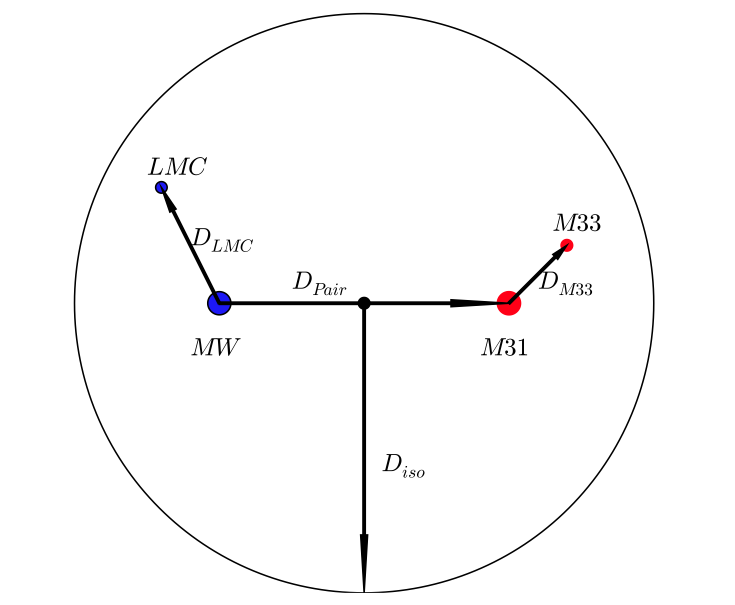
\includegraphics[width=\linewidth]{figures/isd.png}
\caption{2D example of a Quad LG analog. $D_{pair} < 1$ Mpc.  $\DMEE, \DLMC < 0.4$ Mpc.  $D_{iso} < 2$ Mpc.}
\label{fig:iso_diagram}
\end{figure}


\begin{itemize}
\item The distance between the MW and M31 analogs is less than 1 Mpc.  This is ~5 sigma larger than the true value, $D=0.77$ Mpc.
\item Within 2 Mpc of the MW-M31 midpoint, the MW and M31 are the two largest halos.
\item For a given M31 (MW) analog, the associated M33 (LMC) is the most massive halo within 0.4 Mpc.
\end{itemize}
The second criterion enforces that neither MW nor M31 are within the virial radius of a much larger halo.  This is justified by the fact that the Local Group is not part of a larger galaxy cluster. 

\todo{Marc}{Comment on labeling schemes for halos?}




\subsection{Gaussian Mixture Models}
\label{sec:gmm}


We use Gaussian Mixture Models to fit two different distributions in this work: once to fit the likelihood function (henceforth referred to as the LGMM), $\textbf{Pr(d$\vert$x)}$, and once to fit the \consuelo prior (henceforth referred to as the PGMM), $\textbf{Pr(x)}$. 
The GMM fit to the \consuelo prior is presented as an alternative to using the \consuelo halo catalog to approximate the cosmological PDF for halo characteristics. This is a novel approach that allows arbitrarily large fake halo catalogs to be generated, assuming the GMM fits the \consuelo prior well. Details on the GMM method and goodness of fit are presented in 
\Sref{sec:gmm_gof_app} 

% - - - - - - - - - - - - - - - - - - - - - - - - - - - - - - - - - - - - - - 



\subsection{Observational Constraints}
\label{sec:data}

The observational data used to constrain our two and three-halo cosmological models of the Local Group is shown in Table \ref{table:obs}.

\def\arraystretch{1.4}
\capstartfalse
\begin{deluxetable*}{ccccc}[h]
\tabletypesize{\footnotesize}
\tablecaption{\label{table:obs}
\tablewidth{500pt}
Observables of MW, M31, and M33.}
\startdata
\hline
\hline
                     & M31               & M33         &LMC               & Reference          \\
\hline

$\alpha$ / deg          & $ 10.68 \pm 0.08$ & $ 23.46 \pm 0.08$ &$78.76 \pm 0.52$& NED   \\
$\delta$ / deg          & $ 41.27 \pm 0.08$ & $ 30.66 \pm 0.08$ &$-69.19 \pm 0.25$& NED   \\
$D$ / Mpc               & $  0.77 \pm 0.04$ & $ 0.79 \pm 0.23$ &$0.0500 \pm 0.0025$& vdM12, vdM02LMC   \\
$v_{r}$ / km s$^{-1}$  & $ -301.8 \pm 1.00$ & $ 180.0 \pm 1.00$ &$262.0 \pm 3.40$& vdMG08, vdM02LMC   \\
$v_{W}$ / km s$^{-1}$  & $  -125.2 \pm 30.8$ &  N/A & N/A & vdM12   \\
$v_{N}$ / km s$^{-1}$  & $  -73.8 \pm 28.40$ &   N/A & N/A & vdM12   \\
$\mu_{W}$ / $\mu$as yr$^{-1}$ & $  -42.2 \pm 12.30$ & $ 4.70 \pm 3.20$ &$-1910.00 \pm 160.00$& Sohn12, vdMG08, K13   \\
$\mu_{N}$ / $\mu$as yr$^{-1}$ & $  -30.9 \pm 11.7$ & $ -14.1 \pm 6.4$ &$229.00 \pm 160.00$& Sohn12, vdMG08, K13   \\


\hline
\enddata
\tablecomments{
The first two quantities, right ascension and declination, are measured so precisely that the uncertainty can be ignored. $(\mu_{W}, \mu_{N})$ are the proper motions in spherical coordinates, while $(v_{W}, v_{N})$ are the associated linear velocities. The $(\delta v_{rot})$ quantities are a correction for the internal rotation of the galaxies being observed (M31 and M33). This correction is only necessary for calculating the $(v_{W},v_{N})_{M33}$ velocities for M33.  The velocities for M31 are obtained from the literature.
}
\medskip
\end{deluxetable*}
\capstarttrue

As discussed in the section on coordinate transformations, this data is measured in Equatorial coordinates. In order to obtain the parameters used to define a Local Group, $(D, v_{r}, v_{t})_{MW,M33}$, we apply the described coordinate transformations to change to the M31 galactocentric reference frame. 

%%%%%%%%%%%%%%%%%%%%%%%%%%%%%%

%%%%%%%%%%%%%%%%%%%%%%%%%%%%%%



% - - - - - - - - - - - - - - - - - - - - - - - - - - - - - - - - - - - - - - 

% ----------------------------------------------------------------------------
\def\arraystretch{1.4}
\capstartfalse
\begin{deluxetable*}{lccccccc}[h!]
\tabletypesize{\footnotesize}
\tablecaption{\label{table:mass_res}
Log Posterior Masses $\log(M_{vir}/\Msun)$}
\tablewidth{500pt}
\startdata
\hline
\hline
                      & MW               & M31           &M33           & LMC      & LG           &N     &N95\\
\hline 
Quad (GMM prior)   &  $11.94^{+0.13}_{-0.18}$ & $12.11^{+0.19}_{-0.16}$ & $11.23^{+0.29}_{-0.37}$& $11.10^{+0.21}_{-0.25}$ & $12.32^{+0.16}_{-0.15}$ & $4\times 10^{8}$ & $721$\\
Pair (M33, LMC Existence)   &  $11.89^{+0.30}_{-0.32}$ & $12.30^{+0.26}_{-0.34}$ & $11.16^{+0.32}_{-0.27}$ & $11.14^{+0.31}_{-0.26}$&$12.46^{+0.24}_{-0.31}$ &$1\times 10^{7}$ &$8.87\times 10^{4}$\\
Pair (GMM prior)   &  $11.72^{+0.35}_{-0.40}$ & $12.23^{+0.27}_{-0.33}$ & N/A & N/A & $12.38^{+0.24}_{-0.30}$ &$1\times 10^{7}$ &$5.05\times 10^{4}$  \\
\hline
   
\enddata
\tablecomments{
The first column lists the type of isolation criteria used to define a Local Group analog. Quad and Pair are as defined in the text, and M33, LMC Existence indicates that only the existence, not the dynamics, are considered in calculating the Likelihood. $N$ is the unweighted sample size, while $N95$ is the number of LG analogs contributing to $95\%$ of the cumulative likelihood.
}
\medskip
\end{deluxetable*}
\capstarttrue


%%%%%%%%%%%%%%%%%%%%%%%%%%%%%%%%%
\section{Results}
\label{sec:results}

In this section, we present the results for our mass posterior calculations. Our comprehensive results for each type of isolation criteria used in this work are shown in Table \ref{table:mass_res}. 
\Fref{fig:LvsPGMM} shows which regions of the \consuelo prior distribution are significantly weighted by the Likelihood function.

\begin{figure*}
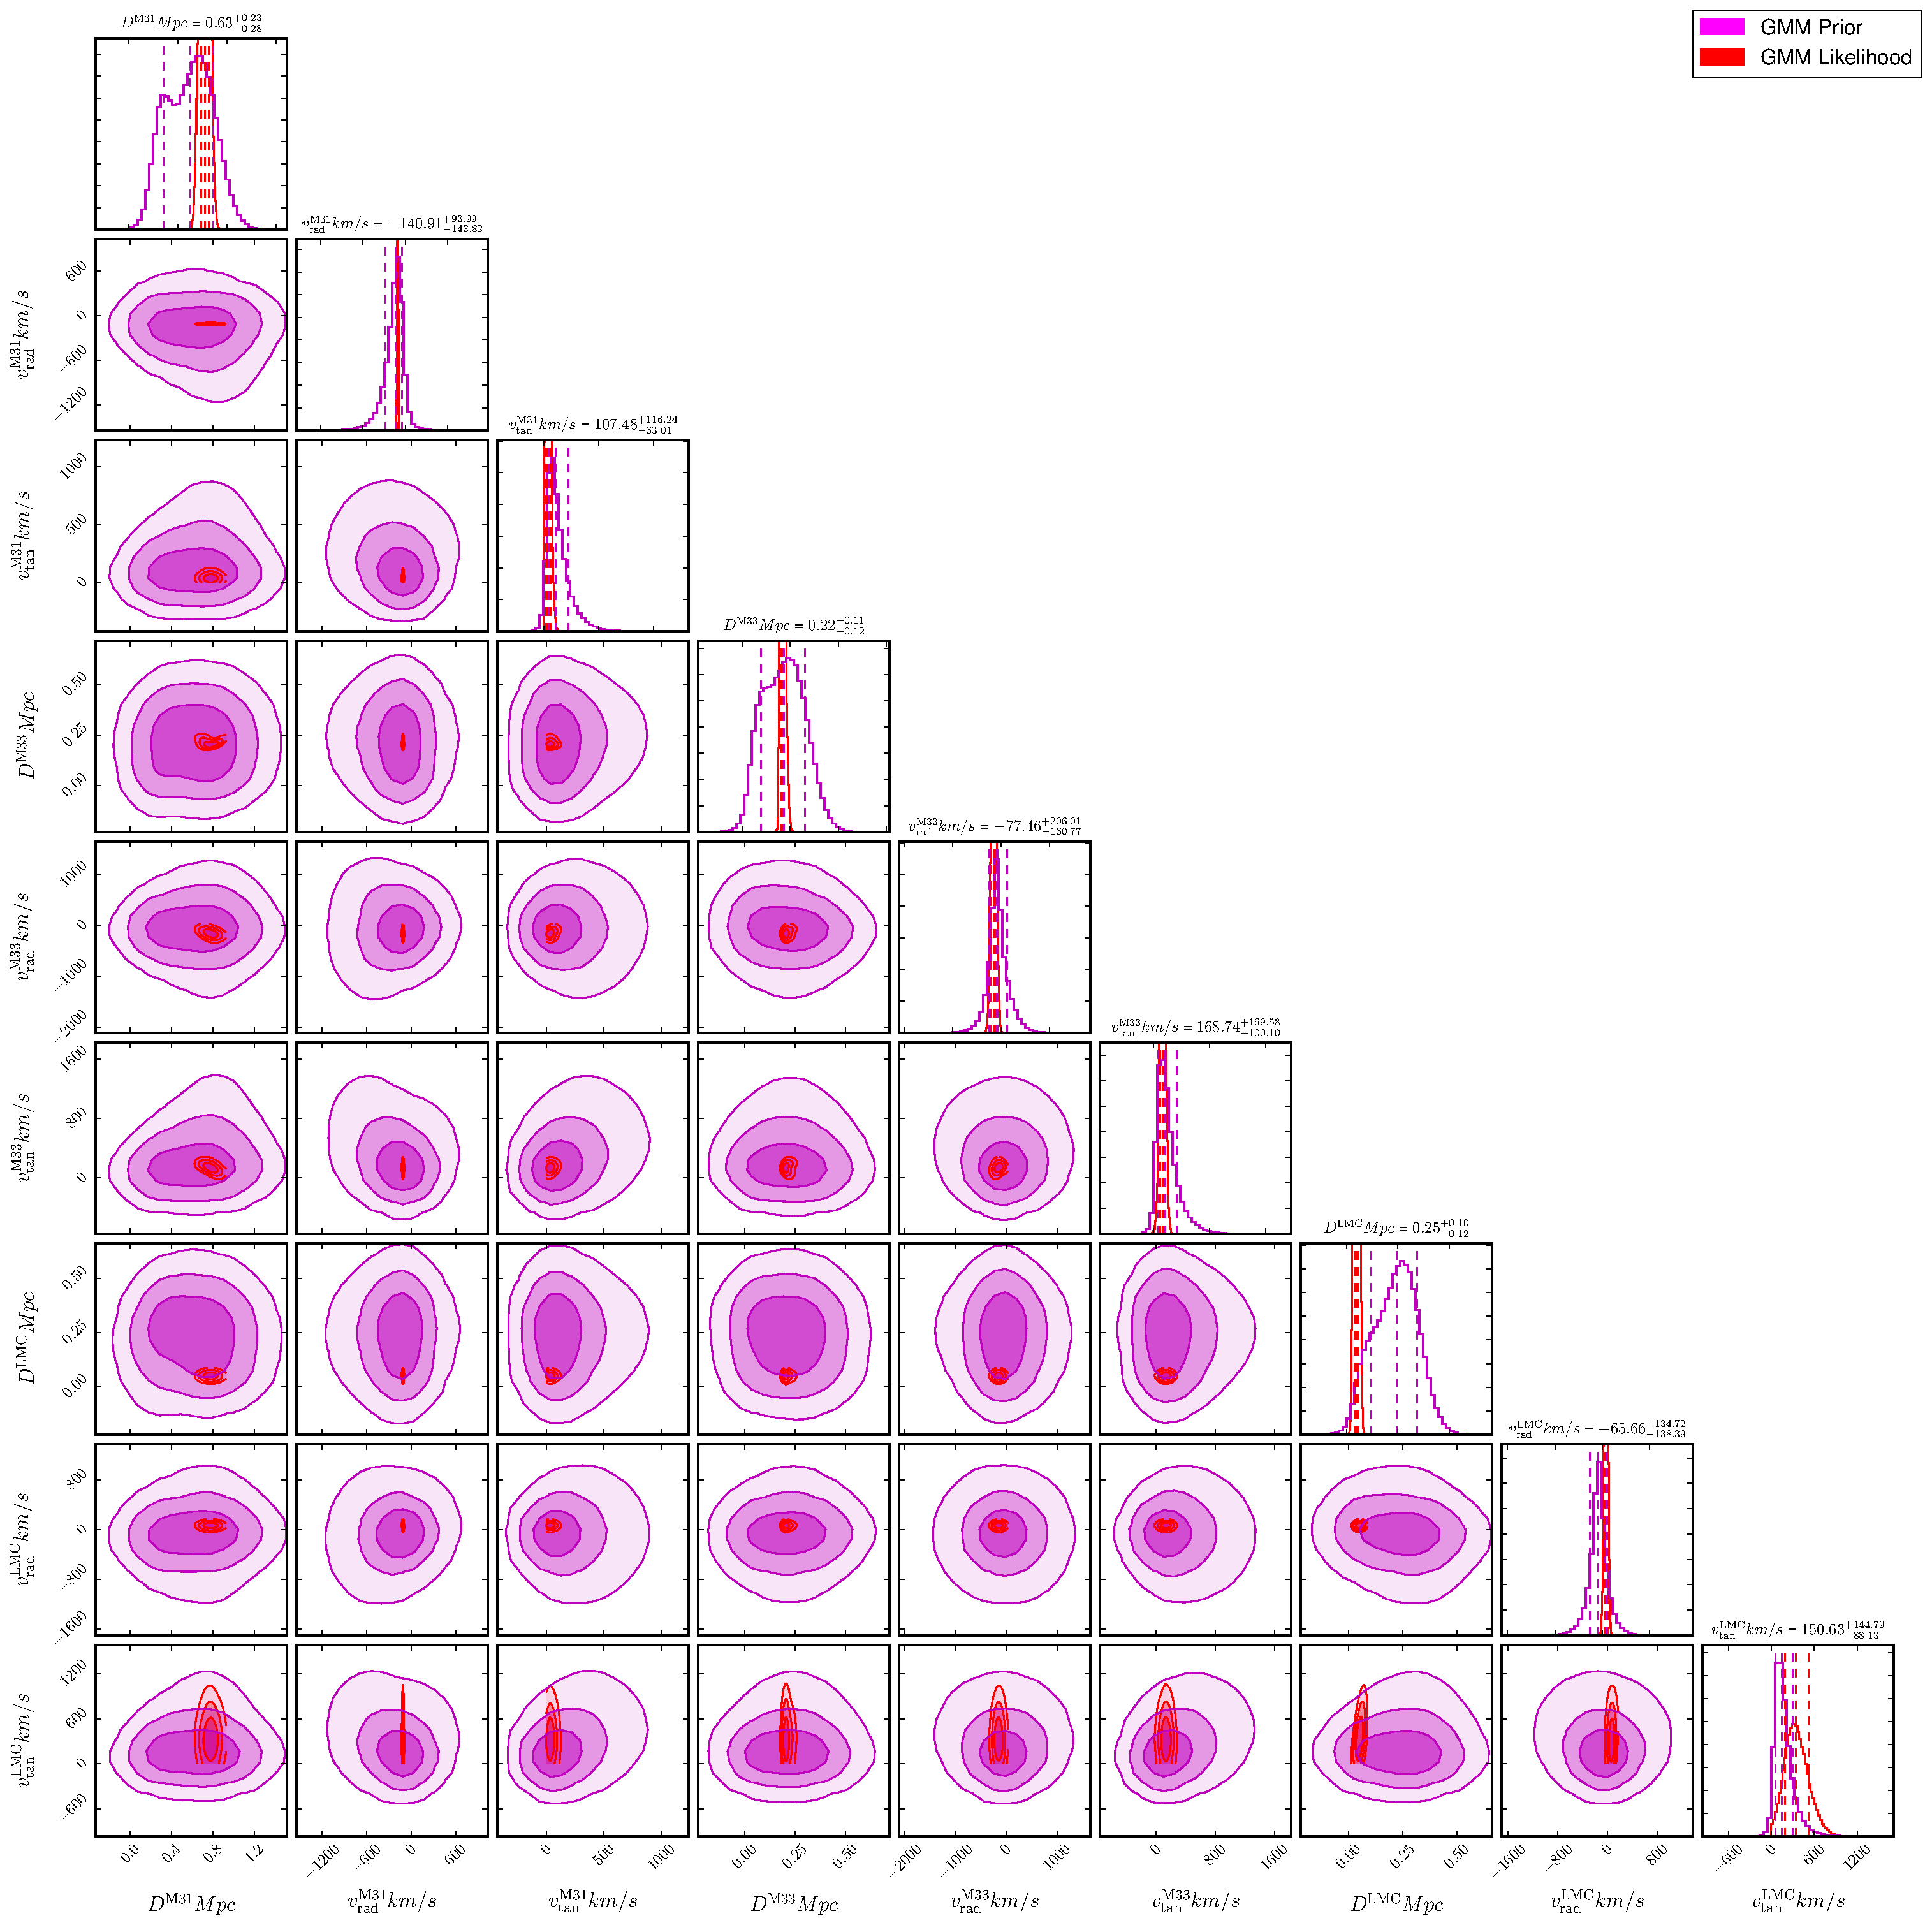
\includegraphics[width=\linewidth]{figures/LvsPGMM.pdf}
\caption{The Quad likelihood contours (red) show which regions of the \consuelo prior are strongly weighted. The LMC uncertainties in proper motion and distance are increased by a factor of four to increase the number of highly weighted Quad systems.}
\label{fig:LvsPGMM}
\end{figure*}



% - - - - - - - - - - - - - - - - - - - - - - - - - - - - - - - - - - - - - - 



\subsection{LG and Halo Masses}
\label{sec:nums}
\Fref{fig:Q_GMMP_all_Mvir} displays the posterior distributions for each of the halo masses in the Quad system. 
The lower mass tails of the LMC and M33 1D histograms show that the halos are resolved in the \consuelo simulations. 
As expected, $\MEI$ correlates strongly with $\MLG$ and $\MMW$.
We find $\MMW = (\MMWestimate^{+\MMWerrorplus}_{-\MMWerrorminus}) \times 10^{12}
\Msun$, $\MLMC = (\MLMCestimate^{+\MLMCerrorplus}_{-\MLMCerrorminus}) \times 10^{12}
\Msun$, $\MEI =
(\MEIestimate^{+\MEIerrorplus}_{-\MEIerrorminus}) \times 10^{12} \Msun$, $\MEE
= (\MEEestimate^{+\MEEerrorplus}_{-\MEEerrorminus}) \times 10^{12} \Msun$, 
and $\MLG = (\MLGestimate^{+\MLGerrorplus}_{-\MLGerrorminus}) \times 10^{12}
\Msun$.
Our estimate for $\MMW$ supports a low Milky Way mass, and our estimate for $\MLMC$ supports a large LMC mass. 

\begin{figure*}[ht]
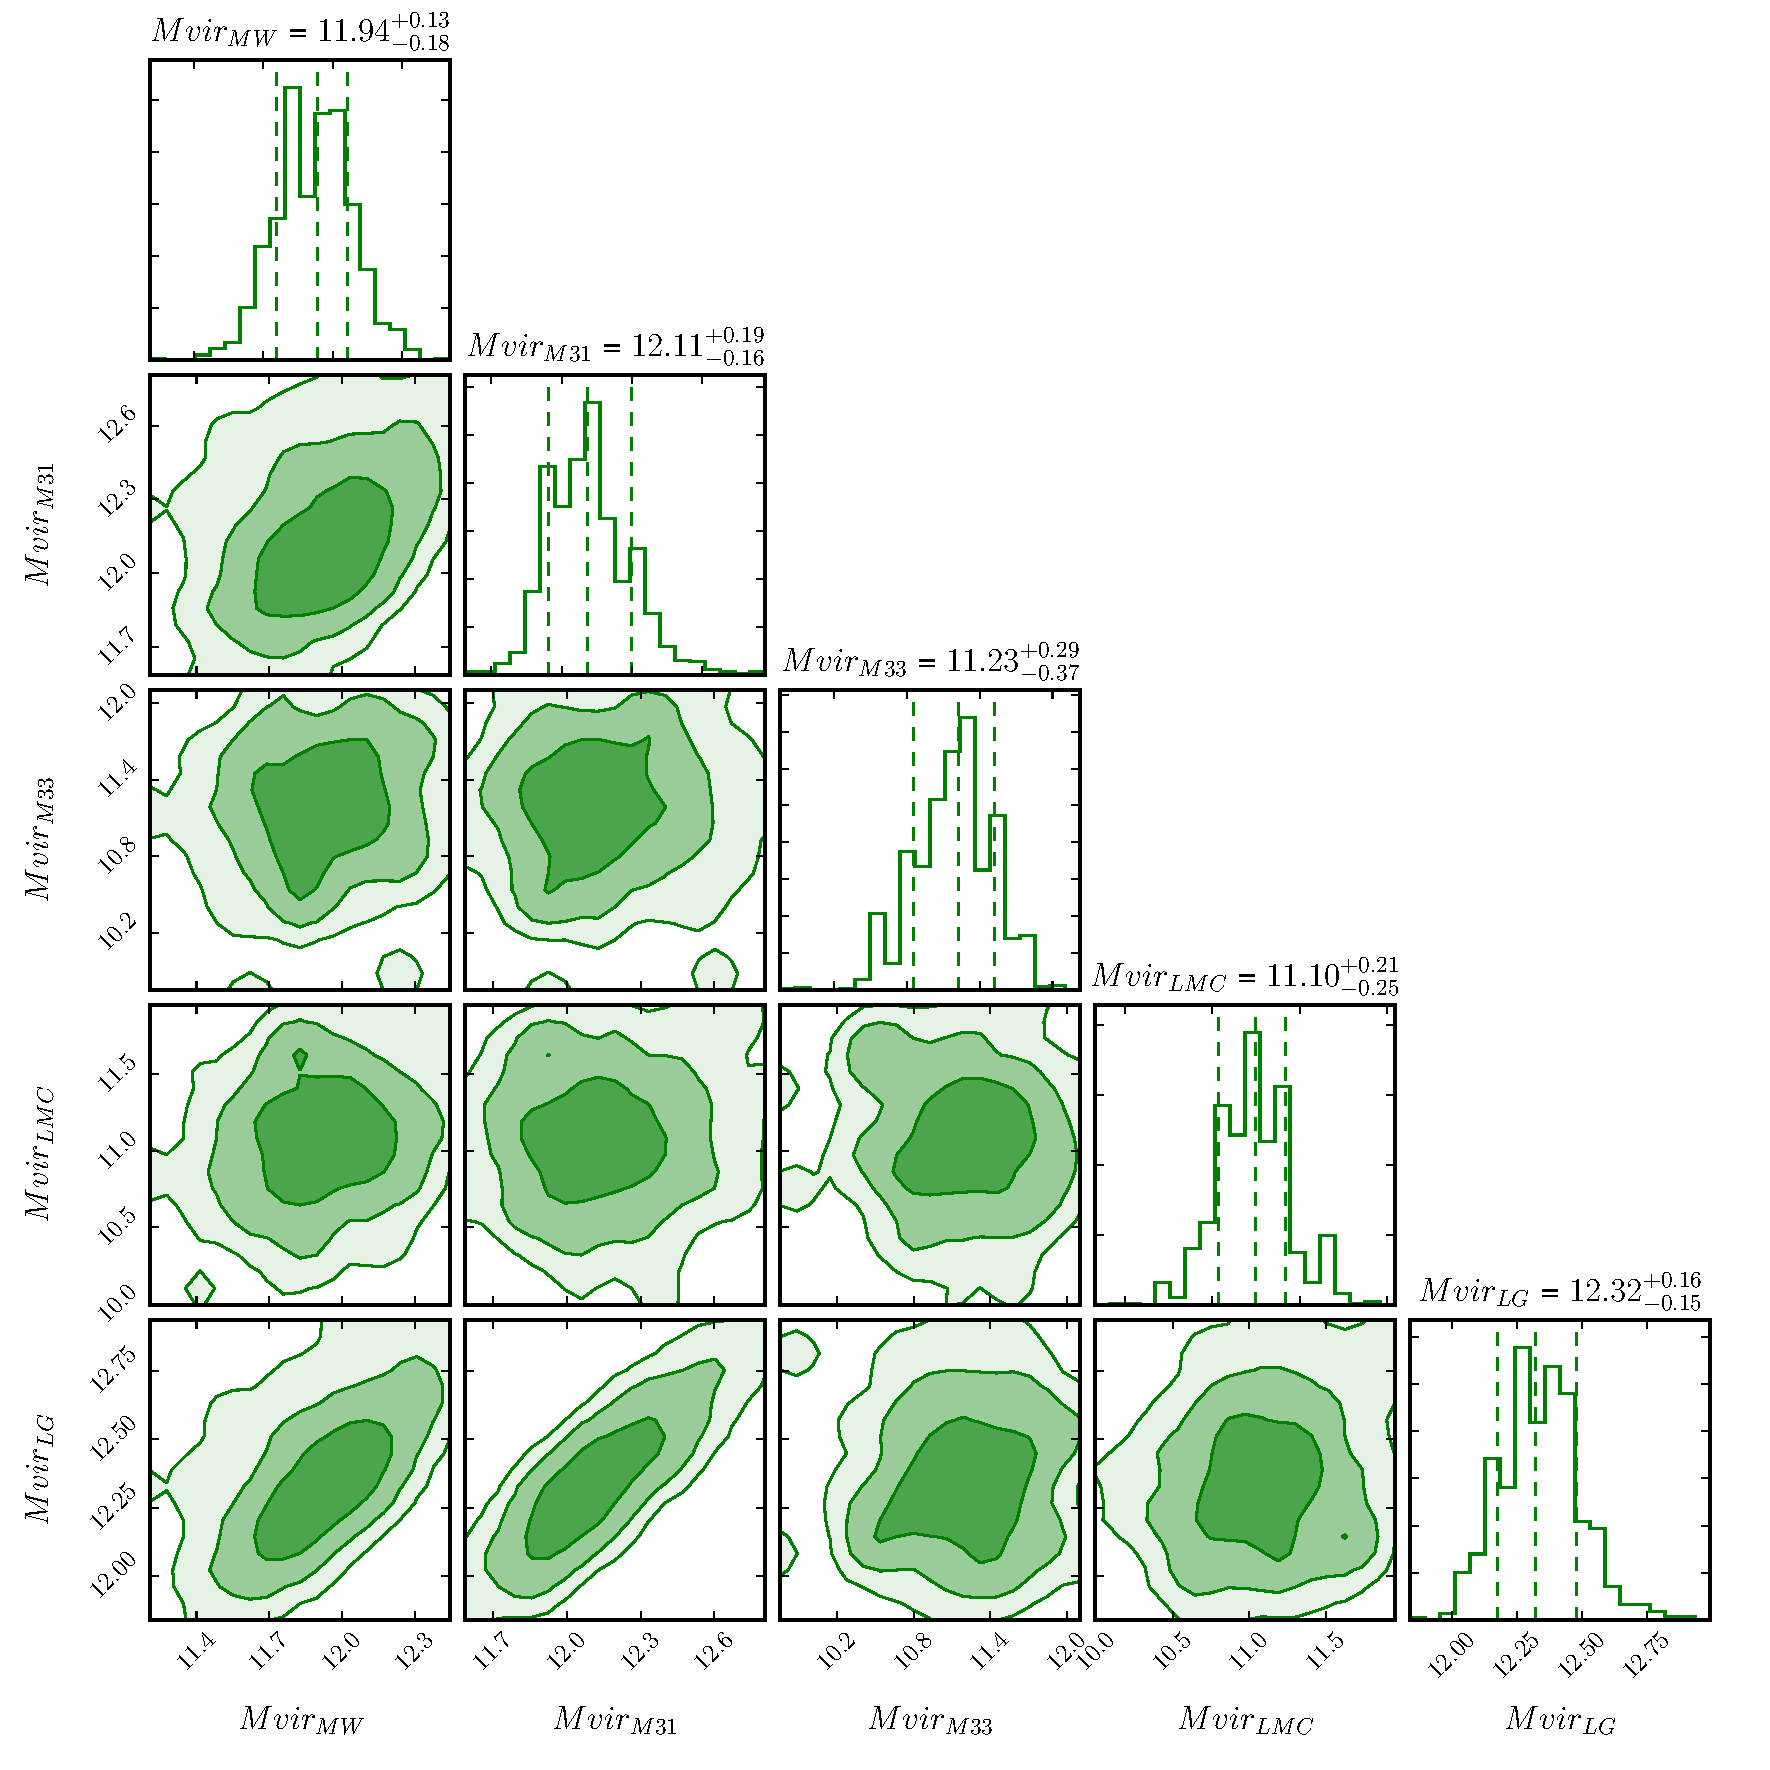
\includegraphics[width=\linewidth]{figures/Q_GMMP_all_Mvir.pdf}
\caption{Posterior distributions of log virial mass for MW, M31, M33, LMC, and the LG, where the LG mass is the sum of MW and M31 masses.}
\label{fig:Q_GMMP_all_Mvir}
\end{figure*}

%\begin{itemize}
%\item Present MW, M31, M33, and LMC masses.
%\item Relative size of MW and M31.
%\item Are LMC and M33 masses resolved? (Are 1D histograms cut off)
%\item Present M200 masses?
%\end{itemize}

\subsection{Halo Concentrations}
\label{sec:conc}
\Fref{fig:Q_GMMP_M31_MvsC} and \Fref{fig:Q_GMMP_MW_MvsC} display the posterior predictions for the concentration-mass relation for M31 and the MW respectively. 
We find 
$\CMW = \CMWestimate^{+\CMWerrorplus}_{-\CMWerrorminus}$ and 
$\CMEI = \CMEIestimate^{+\CMEIerrorplus}_{-\CMEIerrorminus}$. 
The plots also show the prior concentration-mass relation in the relevant mass regime. We note that the posterior 2D distributions show that there is no correlation between mass and concentration for both M31 and the MW. 
This is somewhat surprising, and it indicates that M31 and the MW can have more extreme concentrations for their mass than would be expected from simply analyzing the \consuelo prior.

\begin{figure}[ht]
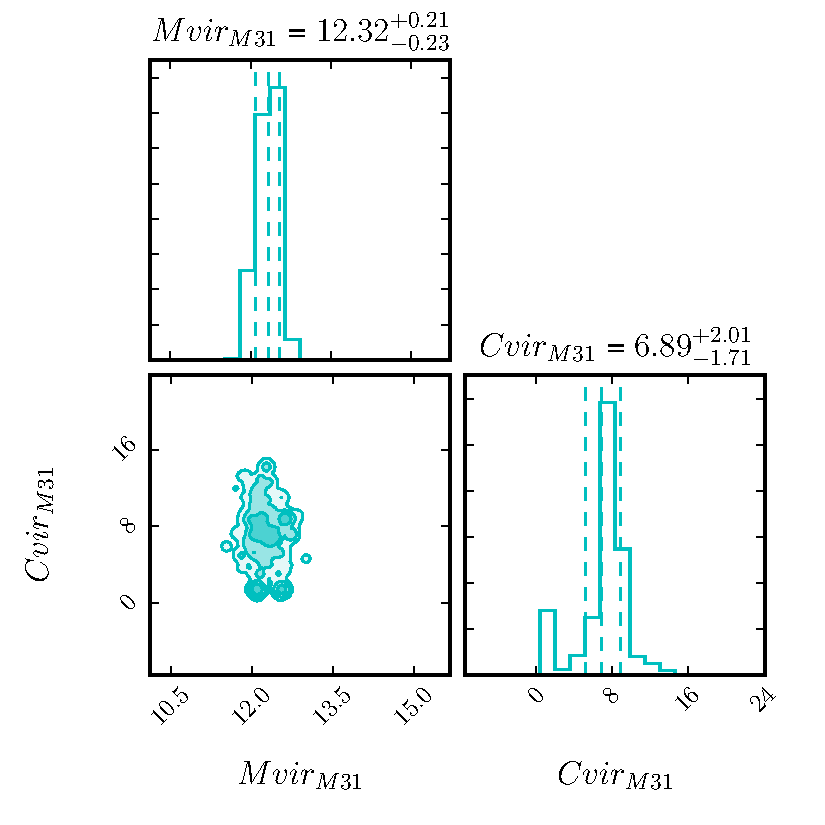
\includegraphics[width=\linewidth]{figures/Q_GMMP_M31_MvsC.pdf}
\caption{Posterior distributions of log mass and concentration for M31. The concentration-mass relation with an uncertainty of $1\sigma$ for this mass regime is shown overlayed.}
\label{fig:Q_GMMP_M31_MvsC}
\end{figure}

\begin{figure}[ht]
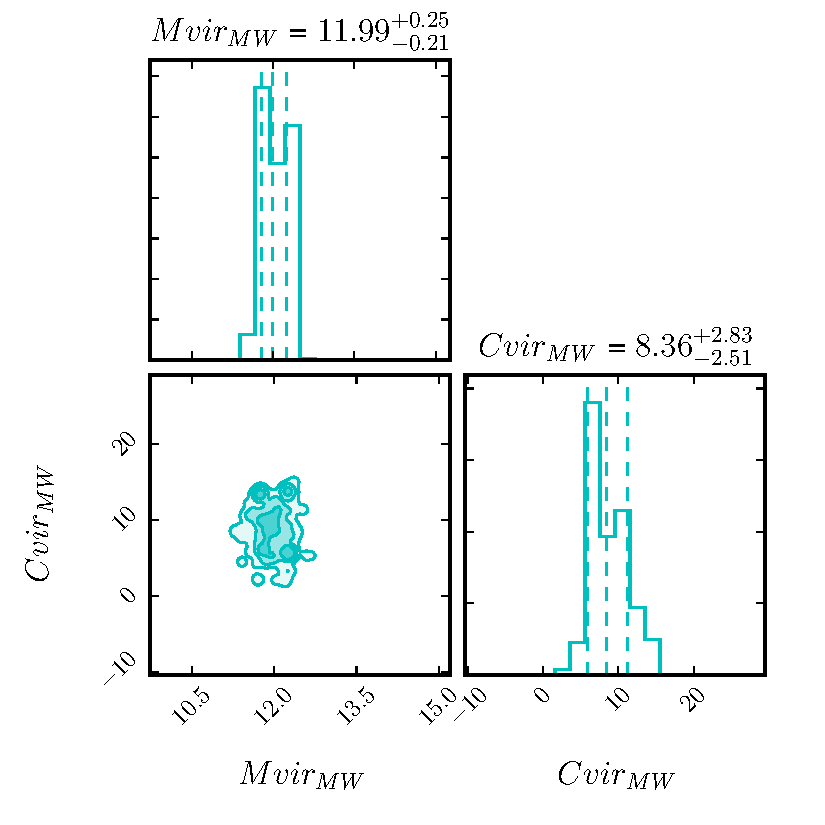
\includegraphics[width=\linewidth]{figures/Q_GMMP_MW_MvsC.pdf}
\caption{Posterior distributions of log mass and concentration for MW. The concentration-mass relation with an uncertainty of $1\sigma$ for this mass regime is shown overlayed.}
\label{fig:Q_GMMP_MW_MvsC}
\end{figure}

%\begin{itemize}
%\item Present MW, M31, M33, and LMC %concentrations.
%\item Mvir-Cvir correlation?
%\item Relative Cvir of MW and M31.
%\end{itemize}


\subsection{The Effect of M33 and LMC}
\label{sec:existence}
\Tref{table:mass_res} shows that the posterior mass predictions are quite sensitive to the existence and kinematics of M33 and the LMC. 
Ignoring both satellites as was done in \cite{gonzalez2014mass} underestimates $\MMW$ and overestimates $\MEI$. These effects almost negate each other for the Local Group mass. \Fref{fig:ta_plot} compares our results to those of the Timing Argument \citep{Timing}. When the kinematics of M33 and the LMC are included as constraints on the LG definition, the TA significantly overestimates the LG mass.
Therefore, the classic two body approach of the Timing Argument \citep{Timing}, even with the modifications to include local environment variables in the Local Group definition from \cite{gonzalez2014mass}, is insufficient to capture the complete behavior of the Local Group.


\begin{figure}[ht]
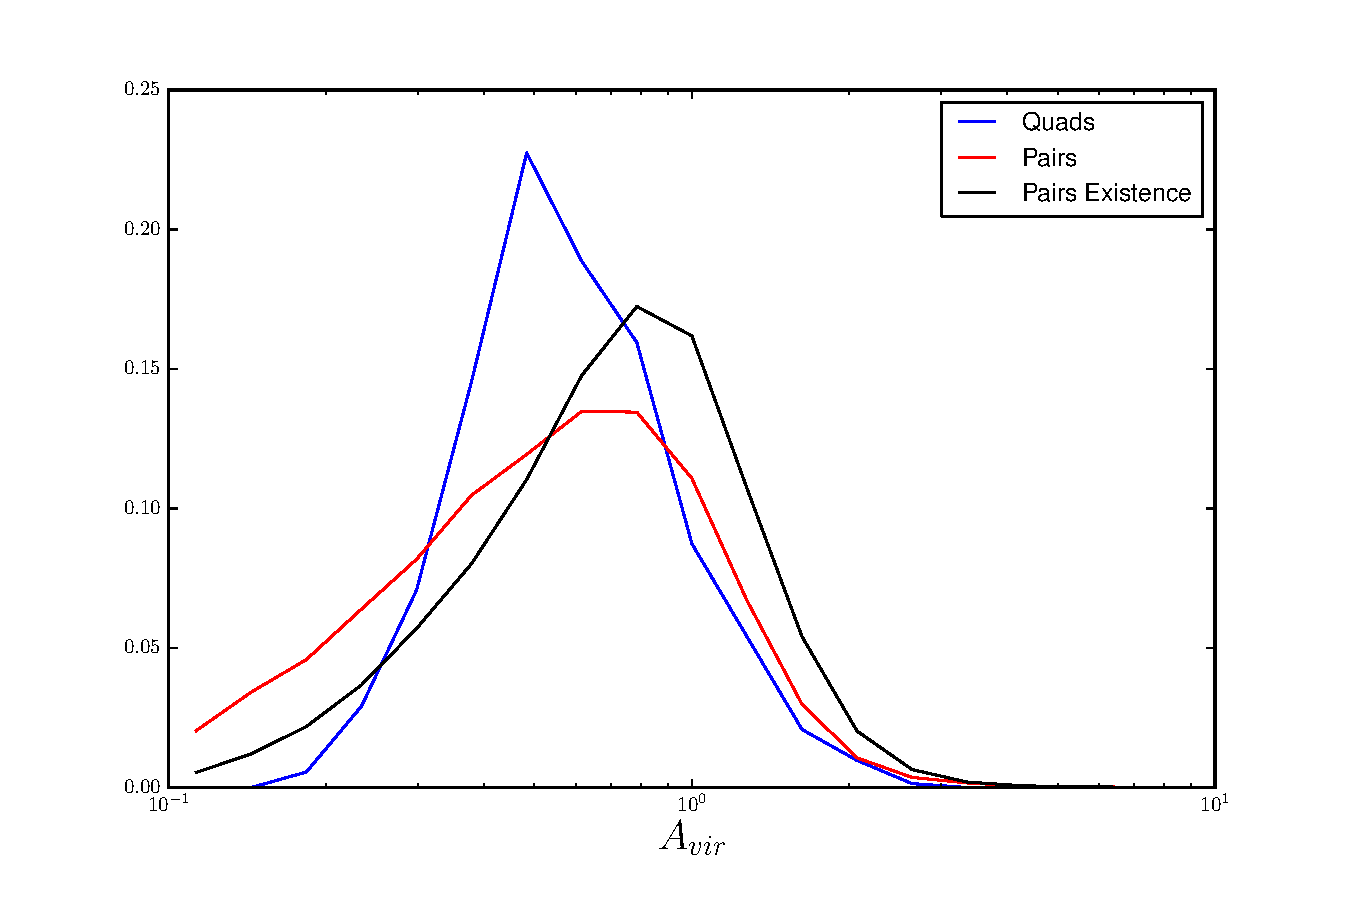
\includegraphics[width=\linewidth]{figures/timing_plot.pdf}
\caption{Ratio of the true MW-M31 pair mass to Timing Argument mass estimate. When only the kinematics of the MW-M31 system are used as constraints, the median of $A_{vir}$ is close to unity. However, when the kinematics of M33 and the LMC are included, the Timing Argument overestimates the LG mass, driving the median of $A_{vir}$ lower.}
\label{fig:ta_plot}
\end{figure}



% ----------------------------------------------------------------------------

\section{Discussion}
\label{sec:discuss}

\subsection{Comparison to the Timing Argument}
\label{sec:TA}

\begin{itemize}
\item Brief summary of TA: Eqs. 1-3 from LW08
\item What did Li and White calculate, and what were their results?
	\subitem LG Mass
	\subitem Bias of the TA
\item Drawbacks of TA
	\subitem Ignores mass evolution
	\subitem Ignores tangential velocity
	\subitem Ignores environment
\item How did Gonzalez et al. update the TA? 
	\subitem Tangential velocity lowers $A_{vir}$.
	\subitem Local density has negligible effect.
\item What do we do differently?
	\subitem Consider the kinematics and existence of M33 and LMC.
	\subitem Make sure to separate the effects of adding LMC and M33 and adding the tangential velocities.
	\subitem Which kinematics are the most important?
\item Figure 6
\end{itemize}

\subsection{Mass of the Milky Way}
\label{sec:MW_discuss}
\todo{Marc}{See what the updated result is for $\MMW$. This will determine what goes in this section.}
\begin{itemize}
\item Brief summary of previous methods. See intro.
\item What do we do differently?
	\subitem M33, LMC
	\subitem compare our results to literature.
	\subitem \subitem Specifically mention differences (and possible problems) with similar methods: Busha, Gonzalez, Kafle, Penarrubia.
\item Consequences for missing satellite problem?
\end{itemize}


\subsection{Mass of LMC}
\label{sec:LMC_discuss}
\todo{Marc}{Update $\MLMC$ value.}
\todo{Marc}{$\MLMC$ lower bound vs $v_{res}$ cut.}
\begin{itemize}
	\item Brief summary of previous models for mass ratio of LMC/MW (see Pena. for sources)
	\item Note use of GMM prior allows us to have enough highly weighted LMC's to get good stats.
	\item Present our calculation of $f_{LMC/MW}$.
		\subitem How does it compare to lit?
		\subitem Consequences of being large?
	\item Is our LMC mass impacted by resolution? By how much?
		\subitem New Figure.
\end{itemize}


\subsection{GMM Prior Goodness of Fit}
\label{sec:gmm_discuss}
\todo{Marc}{Discussion or Appendix?}
\begin{itemize}
	\item What do we use GMM prior for?
		\subitem Why is it important that it must fit distribution well?
	\item GMM prior 1D and 2D marginalizations.
	\item What do we need to check?
		\subitem How much volume (num of consuelo boxes) do we need? New Figure: $\MMW$ post vs GMM volume.
		\subitem How many components in the GMM? New Figure: $\MMW$ post vs num of GMM components.
	\item Pair posterior estimates using GMM prior vs Pair posterior estimates using $\consuelo$.
	\item Implications of good GMM prior.
		\subitem Larger samples
		\subitem Ability to use stronger constraints. 
	
\end{itemize}

Using the Quad definition of the LG, we find that 
$\MEI =
(\MEIestimate^{+\MEIerrorplus}_{-\MEIerrorminus}) \times 10^{12} \Msun$, $\MEE
= (\MEEestimate^{+\MEEerrorplus}_{-\MEEerrorminus}) \times 10^{12} \Msun$,
both of which are consistent at the $1\sigma$ level with previous results \citep{penarrubia2015timing, m33_mass}.
Our posterior constraint on the Milky Way mass, 
$\MMW =
(\MMWestimate^{+\MMWerrorplus}_{-\MMWerrorminus}) \times 10^{12} \Msun$,
is smaller than most previous studies, although still consistent at the $1\sigma$ level with $\MMW = 1.0\times10^{12} \Msun$. 
Since the number of subhalos at a given mass scales with host halo mass \citep{wang2012missing}, a low Milky Way mass is one possible solution to the "Missing Satellite Problem."  Comparing to Figure 5 in Wang et al, we see that there is about a 60 percent chance for a host halo of our mass $\MMW$ to have three or fewer subhalos with $V_{max} > 30$ km/s. 
\par
In addition to finding that the MW is less massive than previously thought, our method shows that the LMC is much larger relative to the MW than expected.  
We calculate the ratio $f_{c} = \MLMC/\MMW$ to be $f_{c} = 0.13^{+0.13 (0.52)}_{-0.05 (0.09)}$, ruling out models where $f_{c} < 0.04$ at the 95 percent level.
Such a large LMC mass relative to the Milky Way could explain the systematic mass overestimate of the Timing Argument seen in \Fref{fig:ta_plot}.
\par
The posterior mass and concentration  calculations presented in this paper depend on the goodness of fit of the PGMM and LGMM, as discussed in \Sref{sec:gmm_gof_app}. 
We find that variations in the number of components in either GMM do not alter the posterior estimates.
As discussed by \cite{kafle2014shoulders}, the MW-LMC point mass approximation affects the posterior calculations by at most 5 percent.
The uncertainties reported in this paper are purely statistical errors.
\par
The work in this paper can easily be extended in numerous ways. 
We have shown that a simple application of unsupervised machine learning (GMM's) can solve small number statistics problems often encountered in working with cosmological simulations.
Other types of learning algorithms (clustering, regression, etc) should be explored.
In this paper, we focus on studying halo mass and concentration. 
There are many other halo properties that could give valuable insight into evolution of the Milky Way and Local Group.
Given how large the large mass of the LMC compared to the MW, it would be interesting to know about the pair's relative orientation and angular momentum.


\section{Summary}
\label{sec:conclude}
\todo{Marc}{Update Summary as results are updated.}
\par
This paper uses the galactocentric kinematic properties of the Local Group to infer the masses of the MW, LMC, M31, and M33. 
We apply a Bayesian method to model the likelihood of a simulated system of halos being a Local Group and use the likelihood to weight a sample of LG analogs drawn from the \consuelo prior. 
This allows us to derive posterior PDF's for any halo property tracked by the simulation, most notably halo mass and concentration. 
We present a novel use of Gaussian Mixture models to approximate the prior halo PDF, allowing us to surpass current computational limits on the number of halos that it is possible to simulate.
The GMM prior approximation enables the use of M33 and the LMC's kinematics as constraints on the definition of the Local Group for the first time.
\acknowledgments{Acknowledgments go here.}

\bibliographystyle{apj}
\bibliography{references}
\clearpage


\appendix
\section{Coordinate Transformations}
\label{sec:coord}
In this section we describe the coordinate systems used in this paper and present the transformations between them.  As mentioned in the introduction, this work uses the galactocentric dynamics of the MW-M31-M33-LMC system to define a LG analog. Specifically, we use the parameters $\distance$, $\vrad$, and $\vtan$ of M31 and LMC measured in the MW galactocentric frame, and the same parameters for M33 measured in the M31 galactocentric frame. 
The observed values of properties like position, distance, and proper motion for these galaxies are made in equatorial coordinates.  However, the corresponding properties in the \consuelo catalogs are measured in galactocentric coordinates.  Therefore, it is necessary to convert the observations of M31 and LMC to the MW galactocentric reference frame, and the observations of M33 to the M31 galactocentric reference frame.  The rest of this section defines the intermediate coordinate systems used in this work and the coordinate transformations between them.

\subsection{Coordinate System Definitions}
\label{sec:c_sys_defs}
Three types of coordinate systems are used in this work: Geocentric Equatorial, Heliocentric Galactic, and Galactocentric.  Before we describe the mathematical transformations between these systems, it is important to thoroughly understand the definitions of the systems. 
\par The equatorial system is centered on the Earth and based on the concept of a celestial sphere (ie all stars are projected onto a sphere of infinite radius centered on the Earth). Two angles characterize the positions of objects on the celestial sphere: right ascension and declination. Right ascension, $\alpha$, is the angle measured eastwards along the celestial equator between the vernal equinox and the hour circle passing through an object.  Declination, $\delta$, is the angular distance of an object above or below the celestial equator.  

\begin{figure}[ht]
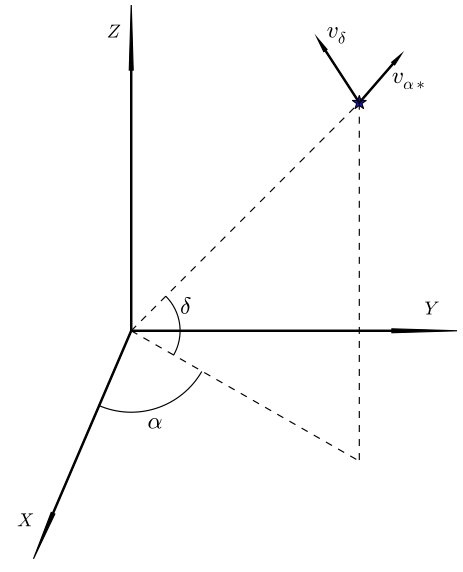
\includegraphics[width=\linewidth]{figures/eq_sys.png}
\caption{Illustration of the equatorial coordinate system. The origin is the center of the Earth. The $X$ axis points towards the Vernal Equinox; the $Y$ axis points 90 degrees to the East of the $X$ axis, making the $XY$ plane the plane of the equator; The $Z$ axis points towards the North Pole. Right ascension $\alpha$ and declination $\delta$ are shown, in addition to the proper motions in their respective directions at the position of the measured galaxy.}
\label{fig:eqsys}
\end{figure}

\par The heliocentric galactic coordinate system (often ambiguously referred to as galactic coordinates), is a different spherical coordinate system centered at the Sun.  The heliocentric fundamental plane is aligned with the galactic plane, and the primary direction is along the line connecting the sun and the galactic center.  Positions are measured in galactic latitude and longitude. Latitude, $b$, measures angular distance of an object perpendicular to the galactic plane, with positive angles to the north galactic pole. Longitude, $l$, is the angular distance measured eastward along the galactic equator from the galactic center.

\begin{figure}[ht]
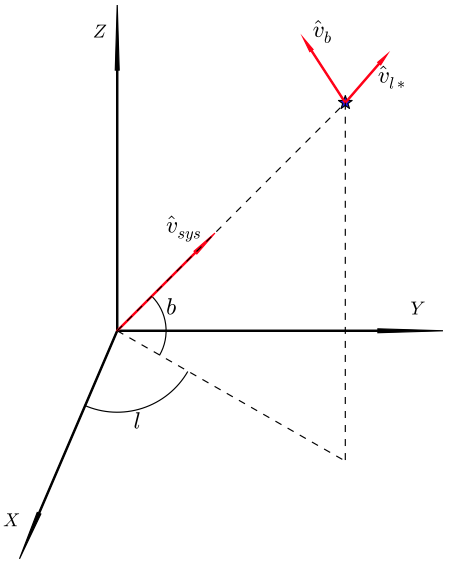
\includegraphics[width=\linewidth]{figures/hel_sys.png}
\caption{Illustration of the heliocentric coordinate system. The origin is the center of the Sun. The $X$ axis points towards the center of the MW; the $Y$ axis points in the direction of the sun's rotation about the galactic center; The $Z$ axis points towards the galactic North Pole. Galactic longitude $l$ and latitude $b$ are shown, in addition to the proper motions in their respective directions at the position of the measured galaxy. $\hat{v}_{sys}$ shows the unit vector in the direction of systemic line of sight velocity for the observed galaxy.}
\label{fig:hel_sys}
\end{figure}

\par The galactocentric coordinate system used in this paper is the same as the one used by van der Marel \citep{VdM08}.  The $Z$ axis points towards the galactic north pole, the $Y$ axis is oriented in the direction of the sun's rotation about the galactic center, and the $X$ axis points from the sun towards the galactic center. This is a standard, right-handed coordinate system. The galactocentric cartesian coordinate system differs from the heliocentric cartesian coordinate system only in the choice of origin, so the transformation between them is a simple translation.

\subsection{Equatorial to Galactic Transformation}
\label{sec:eq_to_gal}
\par 
We require two transformations from Equatorial to Galactic coordinates: one for the positions $(\alpha, \delta)\rightarrow (l,b)$ and one for the proper motions $(\mu_{\alpha*}, \mu_{\delta})\rightarrow (\mu_{l*}, \mu_{b})$. For both transformations, we follow the method described by \cite{poleski2013}, solving the following system of equations to find the Galactic coordinates:
\begin{equation}
\begin{aligned}
\sin b &= \cos\delta\cos\delta_{G}\cos(\alpha - \alpha_{G}) + \sin\delta\sin\delta_{G} \\
\sin(l_{\Omega} - l)\cos b &= \cos\delta\sin(\alpha - \alpha_{G}) \\
\cos(l_{\Omega} - l)\cos b &= \sin\delta\cos\delta_{G} - \cos\delta\sin\delta_{G}\cos(\alpha - \alpha_{G})
\end{aligned}
\end{equation}

where $\alpha_{G} = 192.85948$ and $\delta_{G} = 27.12825$ are the equatorial coordinates of the galactic north pole, and $l_{\Omega} = 32.93192$ is the galactic longitude of the ascending node of the galactic plane.
\par
From Poleski, the transformation for the proper motion is:
\begin{equation}
\left( \begin{array}{c}
\mu_{l*} \\
\mu_{b} \\
\end{array} \right) = 
\frac{1}{\cos b}
\left( \begin{array}{cc}
C_{1} & C_{2} \\
-C_{2} & C_{1} \\
\end{array} \right)
\left( \begin{array}{c}
\mu_{\alpha*} \\
\mu_{\delta} \\
\end{array} \right)
\end{equation}
where...
\begin{equation}
\begin{aligned}
C_{1}&=\sin\delta_{G}\cos\delta - \cos\delta_{G}\sin\delta\cos(\alpha-\alpha_{G})\\
C_{2}&=\cos\delta_{G}\sin(\alpha-\alpha_{G})\\
\cos b&=\sqrt[]{C_{1}^2+C_{2}^2}
\end{aligned}
\end{equation}


\subsection{Galactic Spherical to Galactocentric Cartesian}
\label{sec:sphere_to_cart}

As shown in \Fref{fig:hel_sys}, the vectors \textbf{$\hat{v}_{sys}$, $\hat{v}_{l*}$, $\hat{v}_{b}$} form an orthonormal basis for the heliocentric cartesian coordinate system. 
Given the Galactic coordinates $(l,b)$ of an observed galaxy, we can find the orthonormal basis vectors:
\begin{equation}
\begin{aligned}
\mathbf{\hat{v}}_{sys}&=(\cos l\cos b, \sin l\cos b, \sin b)\\
\mathbf{\hat{v}}_{l*}&=\mathbf{\hat{v}}_{sys}\times(-\hat{Z})\\
\mathbf{\hat{v}}_{b}&=\mathbf{\hat{v}}_{sys}\times\mathbf{\hat{v}}_{l*}
\end{aligned}
\end{equation}
The unit vector in the line of sight direction is easily found using trigonometry. The $\hat{v}_{l*}$ unit vector has no $\hat{Z}$ component and must be orthogonal to $\hat{v}_{sys}$. Knowing these two unit vectors determines the value of $\hat{v}_{b}$.
Given this basis, we can use some simple linear algebra to find the Cartesian velocity components. 
Let $\mathbf{v}=(v_{X}, v_{Y}, v_{Z})$ and $\mathbf{\tilde{v}}=(v_{sys}, v_{l*}, v_{b})$. 
Let $M$ be the change of basis matrix with columns equal to the basis vectors above. 
Applying the change of basis formula, we have:
\begin{equation}
\begin{aligned}
\mathbf{\tilde{v}}&=M^{-1}\mathbf{v}\\
M\mathbf{\tilde{v}}&=\mathbf{v}\\
\mathbf{\tilde{v}}^{T}M^{T}&=\mathbf{v}^{T}
\end{aligned}
\end{equation}

The final steps are to correct the velocities for the reflex motion of the sun and to find the galactocentric position with a simple translation. 
We follow the method in \citep{van2002new}, but use the updated values for the position and velocity vectors of the sun.
\begin{equation}
\begin{aligned}
\mathbf{r}_{\odot} &= (-R_{0},0,0)\\
\mathbf{v}_{\odot} &= (U_{\odot}, V_{0}+V_{\odot}, W_{\odot})
\end{aligned}
\end{equation}

where $R_{0} = 8.29\pm 0.16$ kpc and $V_{0} = 239 \pm 5$ km/s are from 
\cite{mcmillan2011mass} 
and the peculiar velocity of the sun with respect to the Local Standard of Rest is $(U_{\odot}, V_{\odot}, W_{\odot}) = (11.1, 12.24, 7.25)$ from 
%\cite{schonrich2010local}. 
The Galactocentric Cartesian position and velocity vectors of the observed galaxy are then:
\begin{equation}
\begin{aligned}
\mathbf{r} &= D\mathbf{\hat{v}}_{sys} + \mathbf{r}_{\odot}\\
\mathbf{v} &= \mathbf{\tilde{v}}^{T}M^{T} + \mathbf{v}_{\odot}
\end{aligned}
\end{equation}

\subsection{MW Galactocentric Observations}
\label{sec:coord_check}
We calculate the Milky Way Galactocentric Cartesian position and velocity vectors of M31, M33, and the LMC and compare to van der Marel's results as a sanity check of our coordinate transformations. 
%\Tref{table:properties} 
shows the results of our calculations. 
Our positions and velocities match those of van der Marel almost exactly.




\def\arraystretch{1.4}
\capstartfalse
\begin{deluxetable}{cccc}[h]
\tabletypesize{\footnotesize}
\tablecaption{\label{table:properties}
\tablewidth{250pt}
MW Galactocentric kinematic properties of M31, M33, LMC.}
\startdata
\hline
\hline
                      & M31               & M33               & LMC          \\
\hline
$\rx$ / Mpc  & $-0.378 \pm 0.019$ & $-0.476 \pm 0.014$ & $-0.001 \pm 0.001$   \\
$\ry$ / Mpc  & $ 0.613 \pm 0.032$ & $ 0.491 \pm 0.014$ & $-0.041 \pm 0.008$   \\
$\rz$ / Mpc  & $-0.283 \pm 0.015$ & $-0.413 \pm 0.012$ & $0.028 \pm 0.006$   \\
$\vx$ / km s$^{-1}$   & $  66.213 \pm 26.893$ & $  43.055 \pm 21.313$ & $-56.519 \pm ???$   \\
$\vy$ / km s$^{-1}$   & $ -76.264 \pm 19.079$ & $ 101.326 \pm 23.424$ & $-224.889 \pm ???$   \\
$\vz$ / km s$^{-1}$   & $  45.008 \pm 26.463$ & $ 138.894 \pm 28.114$ & $220.139 \pm ???$   \\
\hline

\enddata
\tablecomments{
$(\rx,\ry,\rz)$ is a position vector relative to the Galactic center, while
$(\vx,\vy,\vz)$ is a three-dimensional Galactocentric velocity vector. The
components of these vectors were used to derive distances and  radial and
tangential velocities, which are the inputs to the
likelihood calculations in the text. Uncertainties on quantities 
in this table were calculated by Monte
Carlo. For comparison to van der Marel see \citep{vdm12m31} for M31 and M33 and ??? for LMC.
%
%References are:
%vdM02~=~\citet{vanderMarel12}
}
\medskip
\end{deluxetable}
\capstarttrue


\subsection{Note on West and North}
\label{sec:WN}
In the literature, it is common to measure proper motion of galaxies in the North-West coordinate system. This can be confusing because often times authors do not define these directions in the text, but rather in footnotes. Most often, West is the opposite direction of right ascension, $(\mu_{W}=-\mu_{\alpha})$, and North is the same direction as declination.


\section{GMM's}
\label{sec:gmm_gof_app}

In this section, we present a detailed description of the GMM's used in this work and analyze how well they approximate their underlying distributions. 

\subsection{Approximating the Likelihood}
\label{sec:lhood_app}


We use the observables in Table \ref{table:obs} to fit the likelihood function, \LikePR. For the rest of this paper, an ``observed'' Local Group is defined to be a LG system (either Quad or Pair) whose observational properties are consistent with those listed in Table \ref{table:obs}. The properties in Table \ref{table:obs} are assumed to be Gaussian with mean given by the tabular value, and standard deviation given by the uncertainty. For a given ``observed'' LG, its ``observed'' values are drawn from the corresponding Gaussian. In order to fit the likelihood function, we use the following steps:

\begin{enumerate}
\item Draw a large sample of ``observed'' Local Groups.
\item Transform the ``observed'' properties to the relevant (MW or M31) galactocentric frame.
\item Calculate the likelihood parameters, $(D,v_{r},v_{t})$
\item Fit the resulting nine (three) dimensional probability distribution for the ``observed'' Quads (Pairs).
\end{enumerate}

A large ``observed'' LG sample thus gives us the distribution of the likelihood parameters, $(D,v_{r},v_{t})$ for systems similar to the Local Group. In other words, this distribution is $Pr(d\vert x)$ as a function of $x$, where $x=(D,v_{r},v_{t},M_{\text{vir}},C_{\text{vir}},...)$ are the properties of a \consuelo halo and $d$ is the observational data from Table \ref{table:obs}. We fit the above distribution with a Gaussian Mixture Model (GMM) in order to evaluate likelihoods for \consuelo LG analog systems. The GMM has a large number of components because we are only interested in accurately reproducing the probability density function. Thus overfitting is not an issue.


\subsection{Approximating the Prior}
\label{sec:gmm_prior}

Given the isolation criteria, a sample of LG analogs can be found in the \consuelo catalogs.  However, the effective number of samples is determined by the weights assigned to the \consuelo LG analogs. 

In this work, we evaluate the effective number of samples, $N95$, by finding the number of LG analogs that contribute the most to 95 percent of the cumulative likelihood. 
Thus, a large unweighted sample size can effectively only contribute a small number of LG analogs that most resemble the true Local Group. 
This issue is exacerbated by large numbers of constraints in the likelihood function. 

For Quads, an entire \consuelo box contributes only one or two effective LG analogs which is too few to establish tight posterior mass estimates.  
We therefore require a method that can drastically increase the effective sample size without reducing the dimensionality of our likelihood function. 
This is achieved by modeling the \consuelo prior with a high dimensional Gaussian mixture model. The PGMM allows arbitrarily large fake halo catalogs to be drawn. 
\Sref{sec:gmm_gof} discusses how well the GMM's used in this work fit their underlying distributions. A good fit is particularly important for the PGMM.

\subsection{GMM Accuracy}
\label{sec:gmm_gof}

The accuracy of our posterior mass predictions strongly depends on how well the GMM's approximate the respective distributions. Figure \ref{fig:LGMM} shows the LGMM fit to the observed data for Quads. 
The $1\sigma$, $2\sigma$, and $3\sigma$ contours for the LGMM distribution almost perfectly overlap the corresponding contours for the observed data.  Therefore we can confidently conclude that our likelihood model is extremely accurate. 

\begin{figure*}
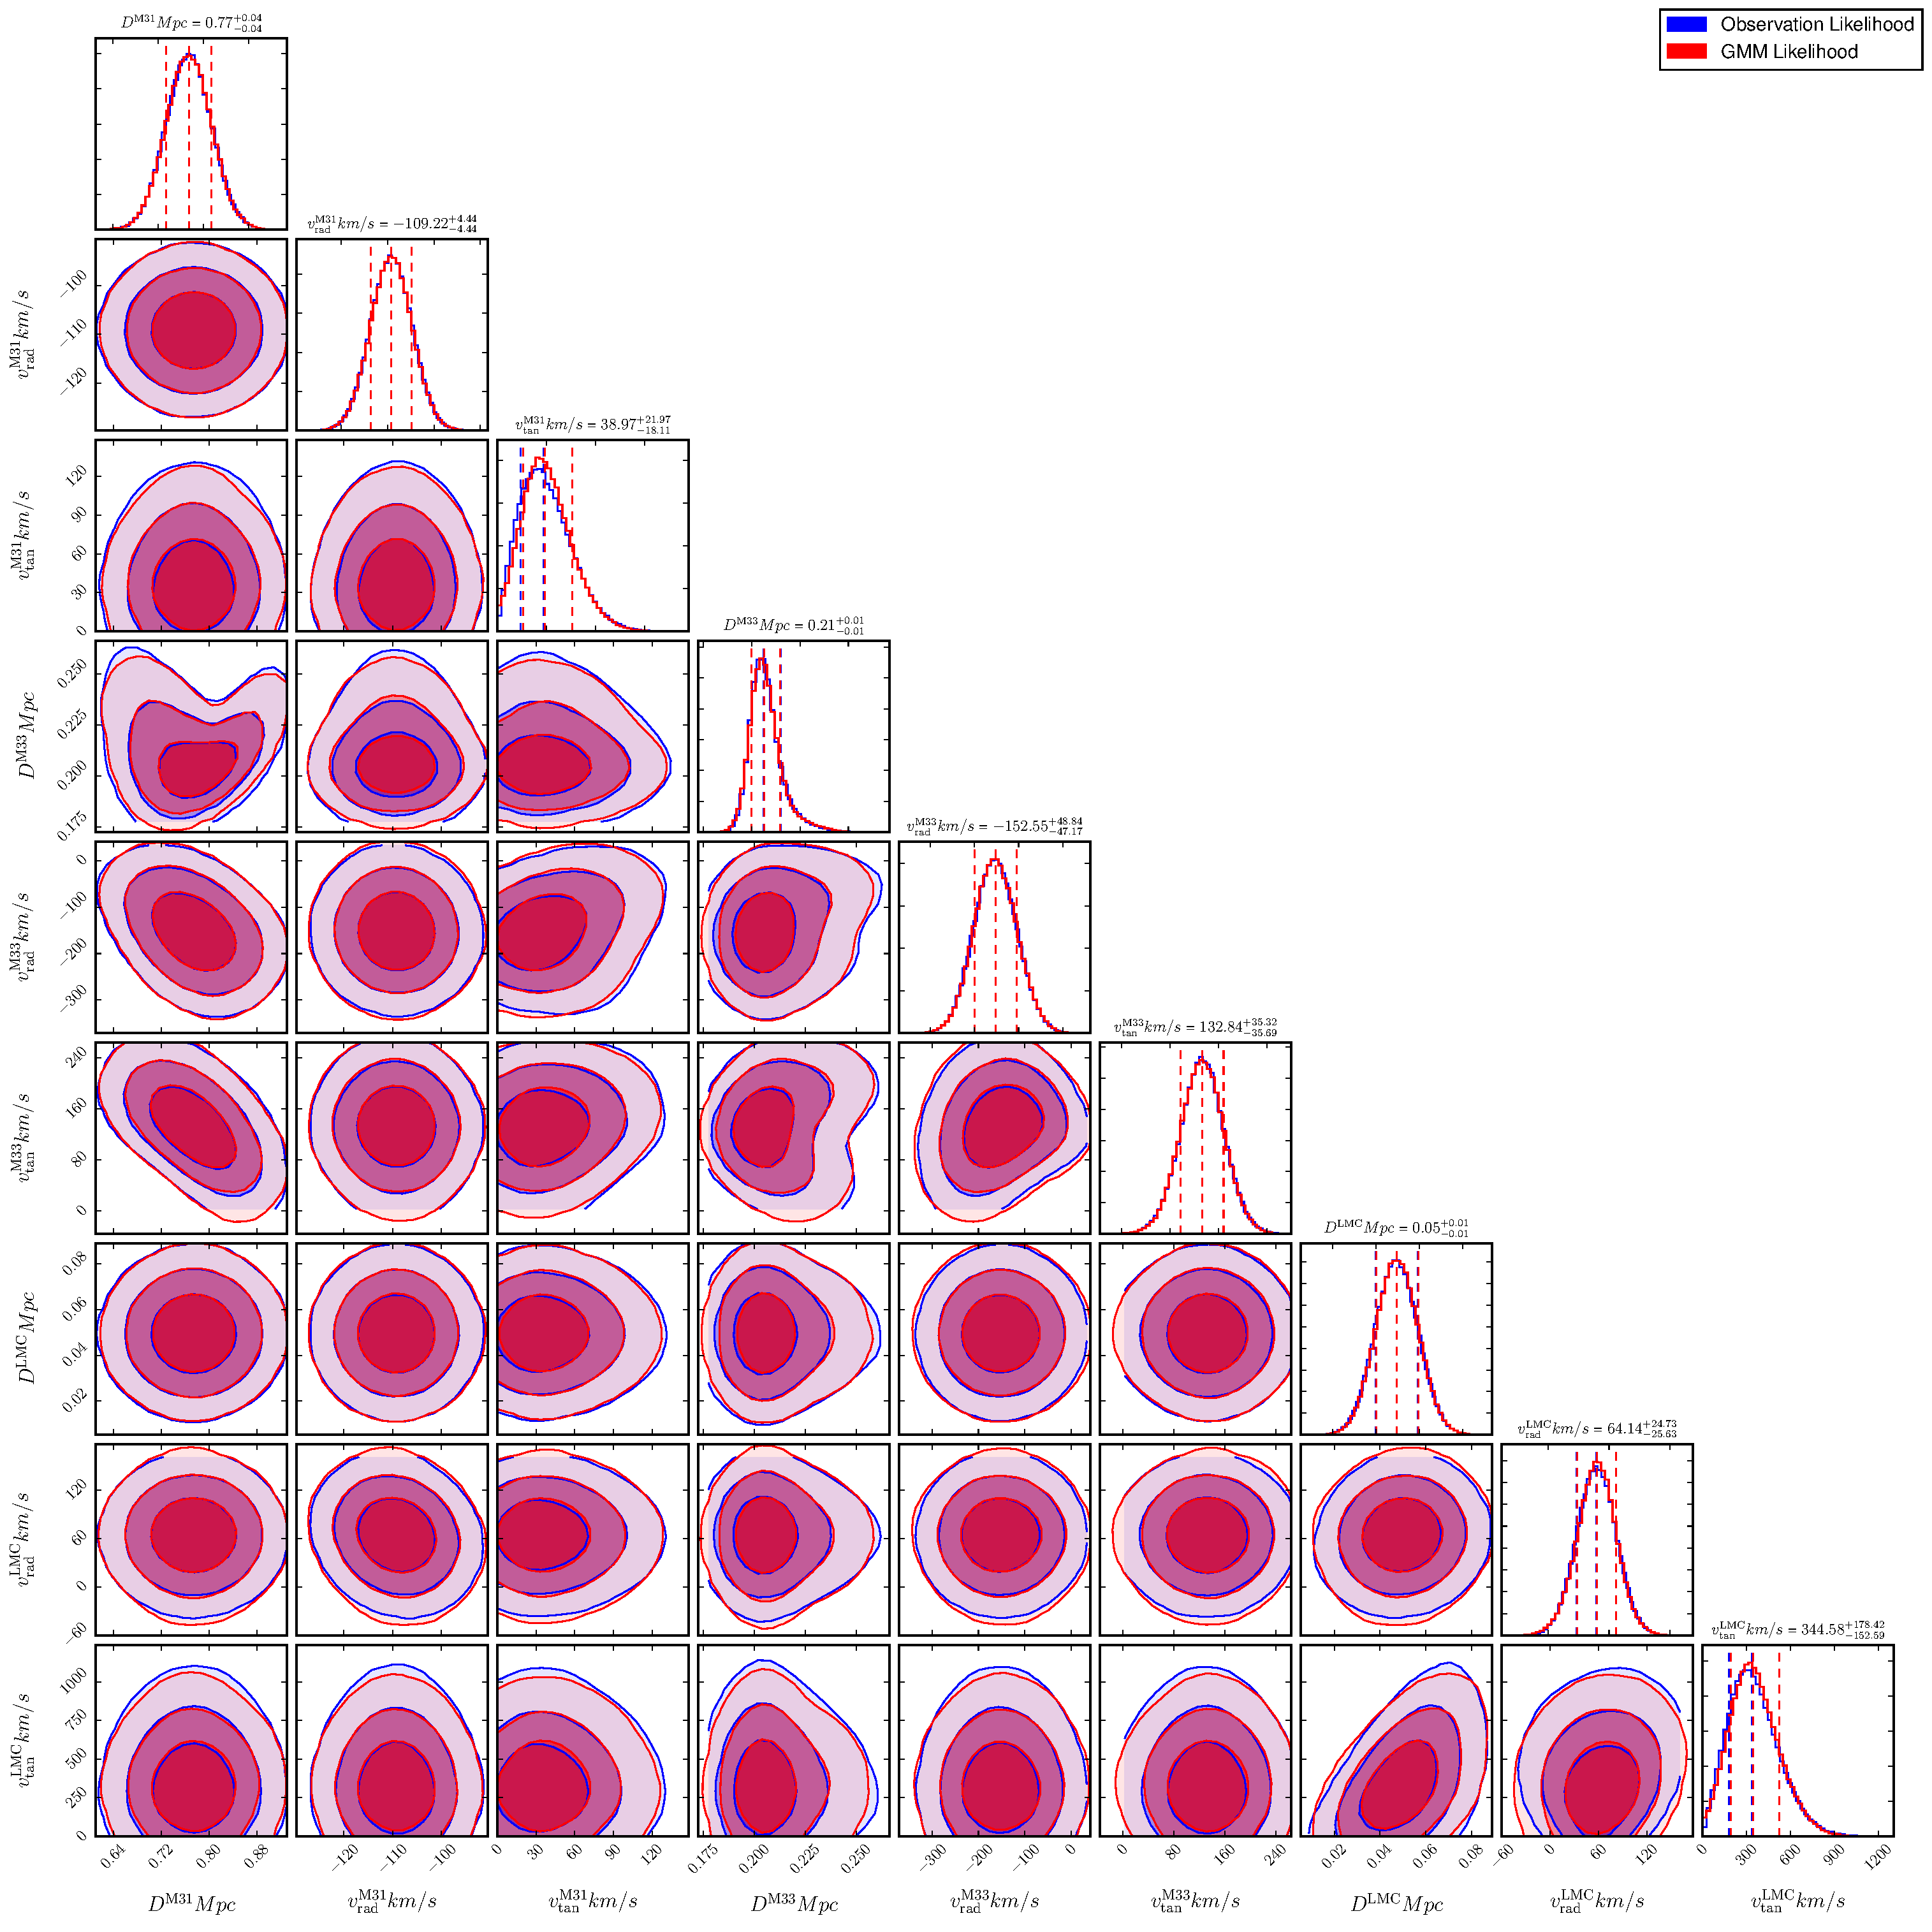
\includegraphics[width=\linewidth]{figures/LGMM.pdf}
\caption{1D and 2D marginalizations of the likelihood function for Quads. The Red contours are generated by the LGMM model and almost perfectly approximate the true distribution.}
\label{fig:LGMM}
\end{figure*}

The second GMM used in this work is the PGMM which models the \consuelo prior. It is particularly important for the model to fit the data extremely well in this case, because we sample directly from the PGMM distribution instead of the true \consuelo prior. Figure \ref{fig:Q_GMMP_GOF} shows the goodness of fit of the PGMM for prior marginalizations. 
As with the LGMM, the $1\sigma$, $2\sigma$, and $3\sigma$ contours almost perfectly overlap. 
This is particularly encouraging for combinations of parameters that are completely independent, like $D^{LMC}$ and $D^{M31}$. 
In this paper, the PGMM has 30 components, and we verify that the posterior estimates do not vary with small changes in the number of components. 
For relatively low dimensional data sets like the ones in this paper, the 1D and 2D marginalizations provide compelling evidence that the PGMM is accurately modeling the \consuelo prior. 
However for high dimensional data sets, the 1D and 2D marginalizations may not be a sufficient goodness of fit test.
In this case, a generalized chi-squared test may be necessary.
Fitting the prior PDF for halo characteristics is a new approach that has not been explored in the literature. 
This method is extremely important because it allows us to create arbitrarily large fake halo catalogs. 
These fake catalogs can contain hundreds of billions of halos, a sample size that is impossible to achieve with current computation limits.
\begin{figure*}
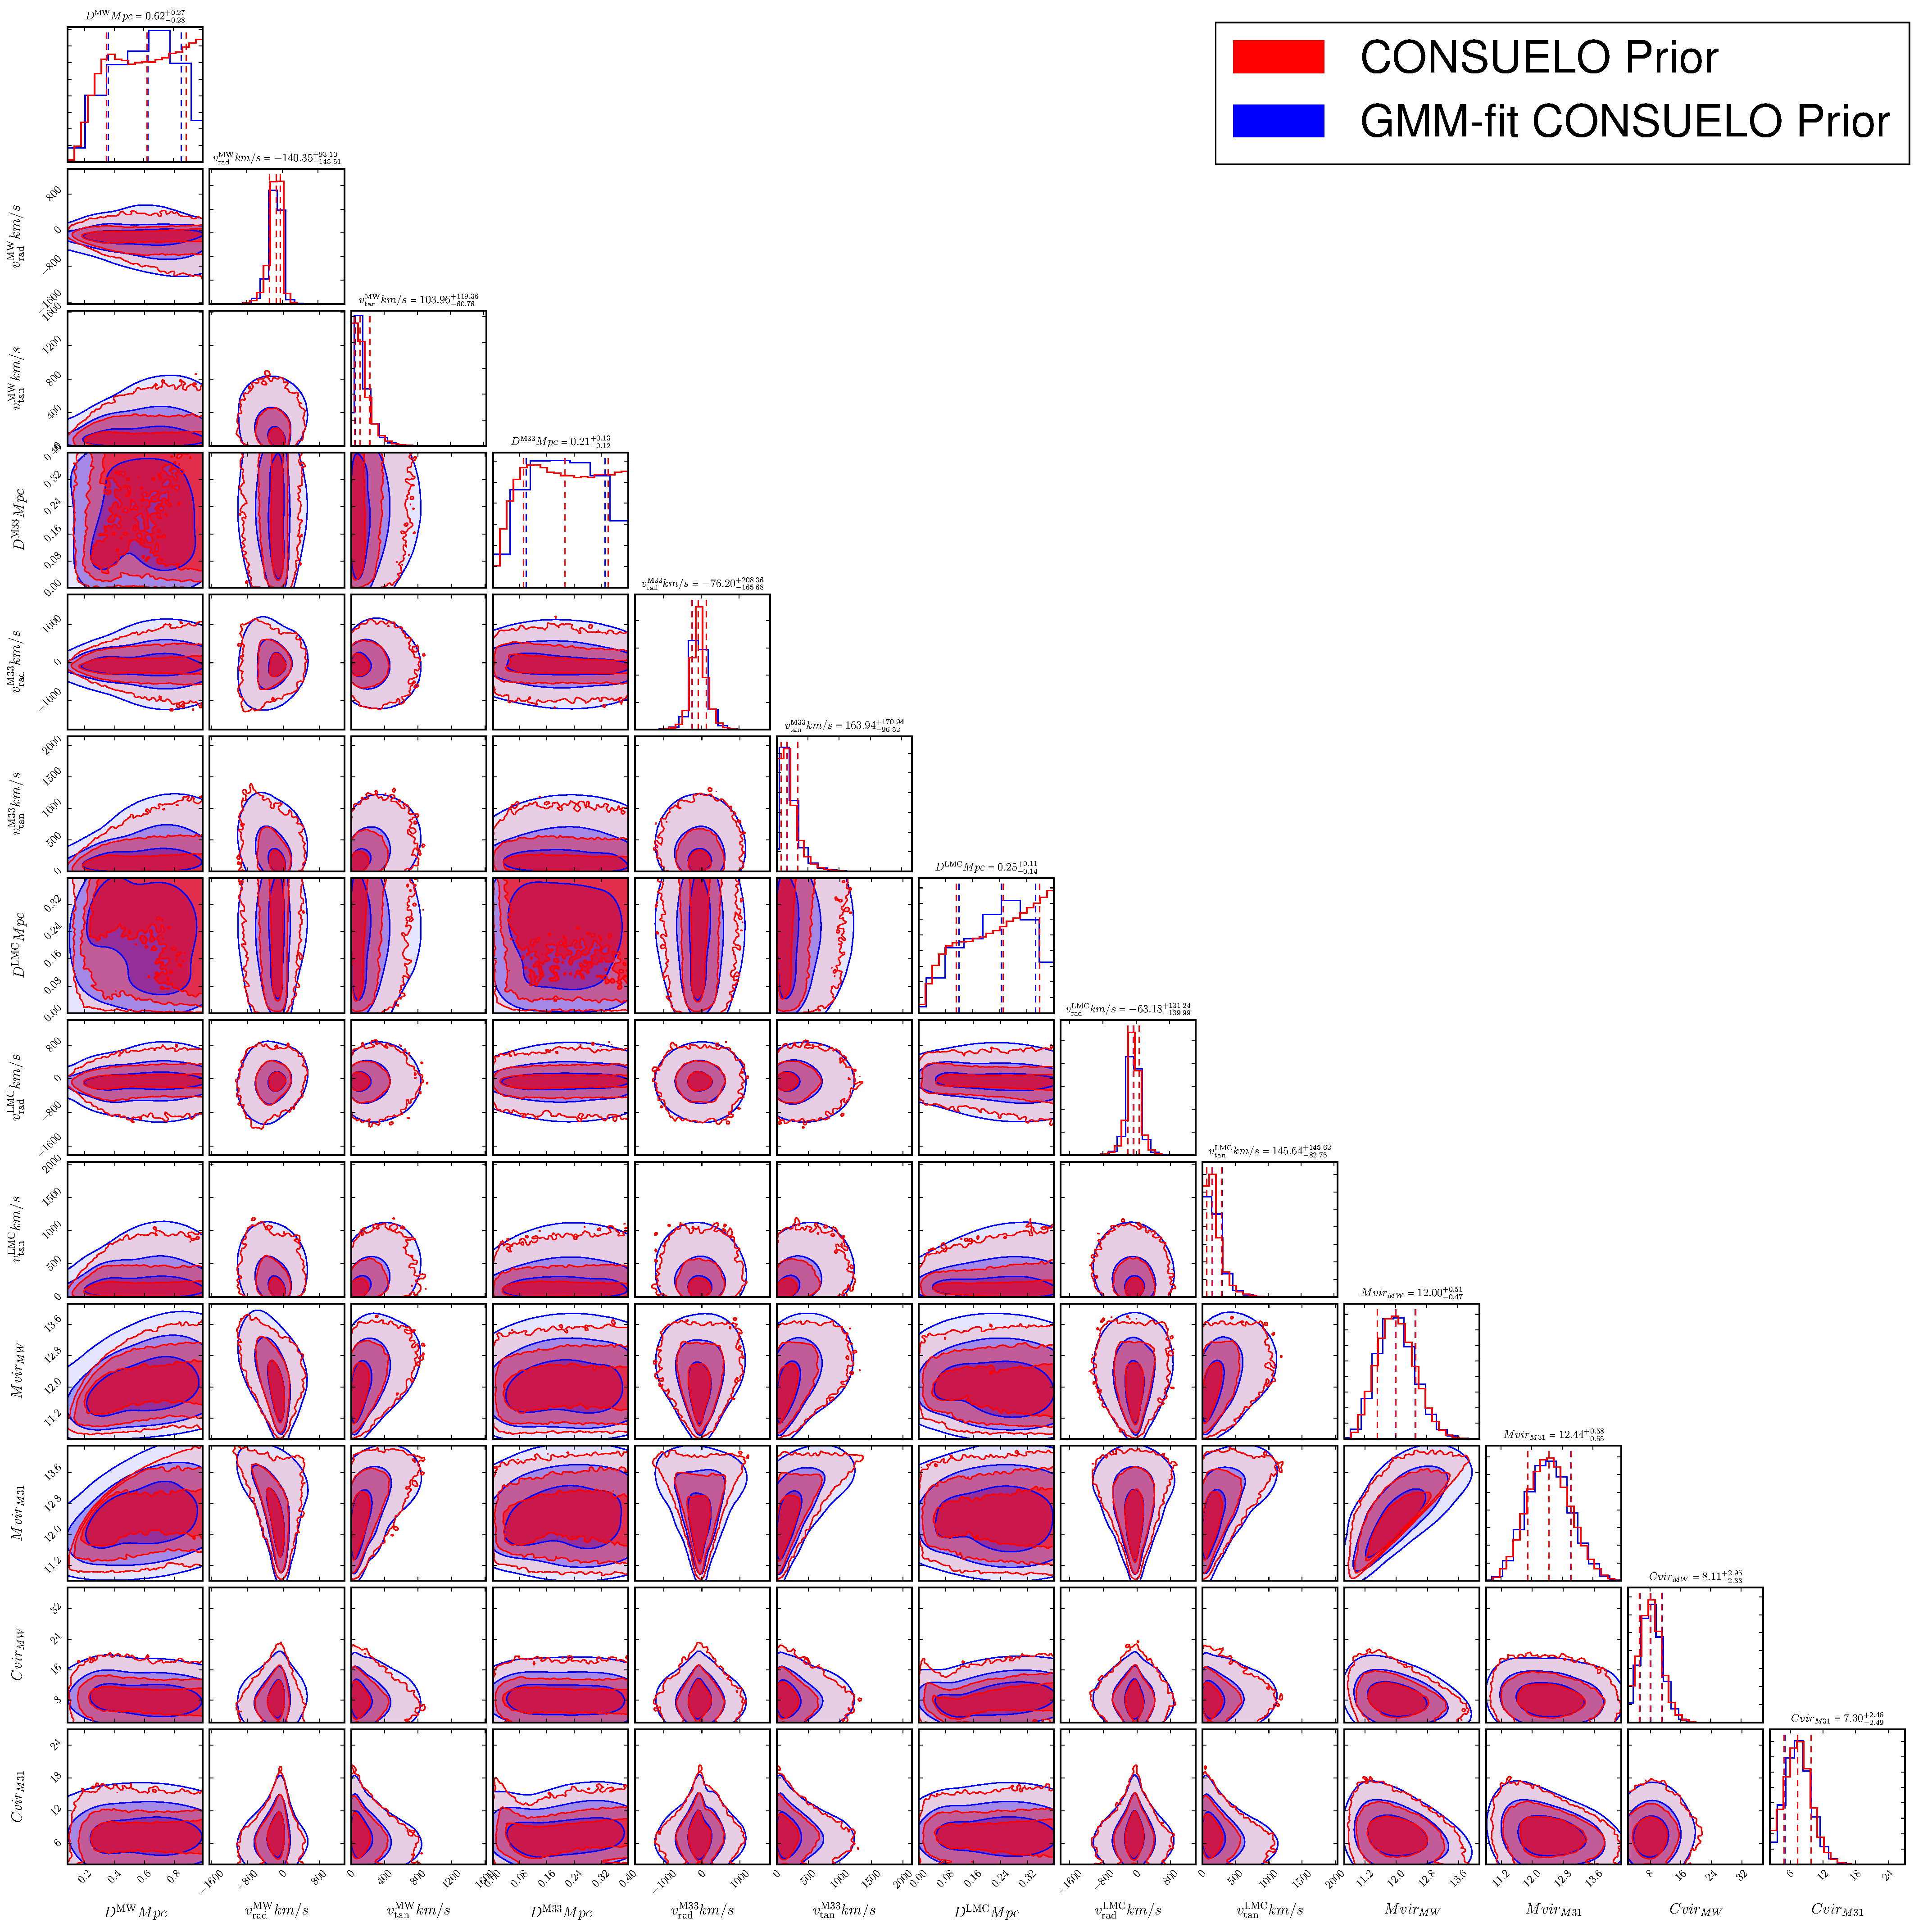
\includegraphics[width=\linewidth]{figures/Q_GMMP_GOF.pdf}
\caption{1D and 2D marginalizations of the Consuelo prior, approximated by the PGMM. The true \consuelo contours (cyan) overlap well with the PGMM contours (magenta).}
\label{fig:Q_GMMP_GOF}
\end{figure*}


\end{document}